%%%%%%%%%%%%%%%%%%%%%%%%%%%%%%%%%%%%%%%%%%%%%%%%%%%%%%%%%%%%%%%%%%%%%%%%%%
%                                                                        %
%  The Why platform for program certification                            %
%                                                                        %
%  Copyright (C) 2002-2011                                               %
%                                                                        %
%    Jean-Christophe FILLIATRE, CNRS & Univ. Paris-sud 11                %
%    Claude MARCHE, INRIA & Univ. Paris-sud 11                           %
%    Yannick MOY, Univ. Paris-sud 11                                     %
%    Romain BARDOU, Univ. Paris-sud 11                                   %
%                                                                        %
%  Secondary contributors:                                               %
%                                                                        %
%    Thierry HUBERT, Univ. Paris-sud 11  (former Caduceus front-end)     %
%    Nicolas ROUSSET, Univ. Paris-sud 11 (on Jessie & Krakatoa)          %
%    Ali AYAD, CNRS & CEA Saclay         (floating-point support)        %
%    Sylvie BOLDO, INRIA                 (floating-point support)        %
%    Jean-Francois COUCHOT, INRIA        (sort encodings, hyps pruning)  %
%    Mehdi DOGGUY, Univ. Paris-sud 11    (Why GUI)                       %
%                                                                        %
%  This software is free software; you can redistribute it and/or        %
%  modify it under the terms of the GNU Lesser General Public            %
%  License version 2.1, with the special exception on linking            %
%  described in file LICENSE.                                            %
%                                                                        %
%  This software is distributed in the hope that it will be useful,      %
%  but WITHOUT ANY WARRANTY; without even the implied warranty of        %
%  MERCHANTABILITY or FITNESS FOR A PARTICULAR PURPOSE.                  %
%                                                                        %
%%%%%%%%%%%%%%%%%%%%%%%%%%%%%%%%%%%%%%%%%%%%%%%%%%%%%%%%%%%%%%%%%%%%%%%%%%

\documentclass[a4paper,11pt,twoside,openright]{report}
\usepackage{hevea}


\usepackage[pdftex,colorlinks=true,urlcolor=blue,pdfstartview=FitH]{hyperref}

\usepackage[latin1]{inputenc}
\usepackage[T1]{fontenc}
\usepackage{times}
\usepackage{amssymb}
%BEGIN LATEX
\usepackage{graphicx}
%END LATEX
%HEVEA \newcommand{\includegraphics}[2][2]{\imgsrc{#2}}

\usepackage{color}
%\usepackage{mathptm}
%\usepackage{xspace}
\usepackage{makeidx}
\makeindex
\input{./version.tex}

% common Why title page

\newcommand{\whytitlepage}[4]{%
\begin{titlepage}
\begin{center}
~\vfill
\rule\textwidth{0.1cm}\\[0.5cm]
\begin{Huge}\sffamily
#1 % title
\end{Huge}
\\[1cm]
\begin{Large}\sffamily
#2
\end{Large}
\\[0.1cm]
\rule\textwidth{0.1cm}\\[1cm]
Version #3\\[3cm]
#4
\vfill
\today\\
INRIA Team-Project \emph{Proval} \url{http://proval.lri.fr} \\
INRIA Futurs \& LRI, CNRS UMR 8623\\ 
4, rue Jacques Monod, 91893 Orsay cedex, France
\end{center}
\end{titlepage}}

\newcommand{\why}{\textsf{Why}}
\newcommand{\Why}{\why}
\newcommand{\java}{\textsc{Java}\index{Java@\textsf{Java}}}
\newcommand{\Java}{\java}
\newcommand{\krakatoa}{\textsf{Krakatoa}\index{Krakatoa@\textsf{Krakatoa}}}
\newcommand{\Krakatoa}{\krakatoa}
\newcommand{\caduceus}{\textsf{Caduceus}\index{Caduceus@\textsf{Caduceus}}}
\newcommand{\Caduceus}{\caduceus}
\newcommand{\coq}{\textsf{Coq}\index{Coq@\textsf{Coq}}}
\newcommand{\Coq}{\coq}
\newcommand{\pvs}{\textsf{PVS}\index{PVS@\textsf{PVS}}}

%

\newcommand{\kw}[1]{\ensuremath{\mathsf{#1}}}

% types
\newcommand{\bool}{\kw{bool}}
\newcommand{\unit}{\kw{unit}}
%\newcommand{\tref}[1]{\ensuremath{#1~\kw{ref}}}
\newcommand{\tref}[1]{\ensuremath{#1~\mathsf{ref}}}
\newcommand{\tarray}[2]{\ensuremath{\kw{array}~#1~\kw{of}~#2}}

% constructs
\newcommand{\prepost}[3]{\ensuremath{\{#1\}\,#2\,\{#3\}}}
\newcommand{\result}{\ensuremath{\mathit{result}}}

\newcommand{\void}{\kw{void}}
\newcommand{\access}[1]{\ensuremath{!#1}}
\newcommand{\assign}[2]{\ensuremath{#1~:=~#2}}
\newcommand{\pref}[1]{\ensuremath{\kw{ref}~#1}}
\newcommand{\taccess}[2]{\ensuremath{#1\texttt{[}#2\texttt{]}}}
\newcommand{\tassign}[3]{\ensuremath{#1\texttt{[}#2\texttt{]}~\texttt{:=}~#3}}
\newcommand{\faccess}[2]{\ensuremath{(\mathit{access}~#1~#2)}}
\newcommand{\fupdate}[3]{\ensuremath{(\mathit{update}~#1~#2~#3)}}
%\newcommand{\taccess}[2]{\ensuremath{#1[#2]}}
%\newcommand{\tassign}[3]{\ensuremath{#1[#2]~:=~#3}}
%\newcommand{\faccess}[2]{\ensuremath{(\mathit{access}~#1~#2)}}
%\newcommand{\fupdate}[3]{\ensuremath{(\mathit{update}~#1~#2~#3)}}
% \newcommand{\block}[1]{\ensuremath{\kw{begin}~#1~\kw{end}}}
\newcommand{\seq}[2]{\ensuremath{#1;~#2}}
%\newcommand{\plabel}[2]{\ensuremath{#1:#2}}
\newcommand{\plabel}[2]{\ensuremath{#1\texttt{:}#2}}
\newcommand{\assert}[2]{\ensuremath{\kw{assert}~\{#1\};~#2}}
\newcommand{\while}[4]{\ensuremath{\kw{while}~#1~\kw{do}~\{\kw{invariant}~#2~\kw{variant}~#3\}~#4~\kw{done}}}
\newcommand{\ite}[3]{\ensuremath{\kw{if}~#1~\kw{then}~#2~\kw{else}~#3}}
\newcommand{\fun}[3]{\ensuremath{\kw{fun}~#1:#2\rightarrow#3}}
\newcommand{\app}[2]{\ensuremath{(#1~#2)}}
\newcommand{\rec}[4]{\ensuremath{\kw{rec}~#1:#2~\{\kw{variant}~#3\}=#4}}
\newcommand{\letin}[3]{\ensuremath{\kw{let}~#1=#2~\kw{in}~#3}}
\newcommand{\raisex}[2]{\ensuremath{\kw{raise}~(#1~#2)}}
\newcommand{\exn}[1]{\ensuremath{\kw{Exn}~#1}}
\newcommand{\try}[2]{\ensuremath{\kw{try}~#1~\kw{with}~#2~\kw{end}}}
\newcommand{\coerce}[2]{\ensuremath{(#1:#2)}}

\newcommand{\statement}{\textit{statement}}
\newcommand{\program}{\textit{program}}
\newcommand{\expression}{\textit{expression}}
\newcommand{\predicate}{\textit{predicate}}

% inference rules
\newcommand{\espacev}{\rule{0in}{1em}}
\newcommand{\espacevn}{\rule[-0.4em]{0in}{1em}}
\newcommand{\irule}[2]
  {\frac{\espacevn\displaystyle#1}{\espacev\displaystyle#2}}
\newcommand{\typage}[3]{#1 \, \vdash \, #2 : #3}
\newcommand{\iname}[1]{\textsf{#1}}

\newcommand{\emptyef}{\bot}
\newcommand{\wf}[1]{#1~\kw{wf}}
\newcommand{\pur}[1]{#1~\kw{pure}}
\newcommand{\variant}[1]{#1~\kw{variant}}

\newcommand{\wpre}[2]{\ensuremath{\mathit{wp}(#1,#2)}}
\newcommand{\wprx}[3]{\ensuremath{\mathit{wp}(#1,#2,#3)}}

\newcommand{\barre}[1]{\ensuremath{\overline{#1}}}

%%% Local Variables: 
%%% mode: latex
%%% TeX-master: "doc"
%%% End: 

\definecolor{darkgreen}{rgb}{0, 0.5, 0}

\setlength{\textheight}{240mm}
\setlength{\topmargin}{-10mm}
\setlength{\textwidth}{160mm}
\setlength{\oddsidemargin}{0mm}
\setlength{\evensidemargin}{0mm}

\renewcommand{\textfraction}{0.01}
\renewcommand{\topfraction}{0.99}
\renewcommand{\bottomfraction}{0.99}

\usepackage{fancyhdr}
\pagestyle{fancyplain}
\renewcommand{\footrulewidth}{0.4pt}
\addtolength{\headheight}{2pt}
\addtolength{\headwidth}{1cm}
\renewcommand{\chaptermark}[1]{\markboth{#1}{}}
\renewcommand{\sectionmark}[1]{\markright{\thesection\ #1}}
\lhead[\fancyplain{}{\bfseries\thepage}]{\fancyplain{}{\bfseries\rightmark}}
\chead{}
\rhead[\fancyplain{}{\bfseries\leftmark}]{\fancyplain{}{\bfseries\thepage}}
\lfoot{\fancyplain{}{C. March\'e}}
\cfoot{\fancyplain{}{Why platform, Krakatoa tool}}
\rfoot{\fancyplain{}{ProVal, \today}}


\begin{document}
\ifhevea%
This document is also available in \ahref{krakatoa.pdf}{PDF format}.
\else
\sloppy
\hbadness=9999
\fi

\whytitlepage{The Krakatoa Verification Tool\\~\\for \Java{} programs}{Tutorial and Reference Manual}{\whyversion}{Claude March\'e}


\tableofcontents

\chapter{Introduction}

Krakatoa is a tool for certification of Java programs, annotated using
the Java Modeling Language~\cite{leavens00preliminary} (JML for
short), using the \Why{}~\cite{why} tool for generating proof
obligations.

This version \whyversion{} of Krakatoa is a major rewriting of
the version 0.x family. Major changes have occurred including changes in the syntax of annotations.

Chapter~\ref{chap:tutorial} is a tutorial to introduce the user step
by step to the use of Krakatoa.

Chapter~\ref{chap:reference} is a reference manual where all options
of the tool are described, and also the modeling of Java objects and
Java memory heap, that you may encounter if you discharge proofs
interactively, e.g. using Coq.

In the appendix you will find various additional informations,
including the requirements, a summary of known limitations, and how to
get help.

\section{Important note for version 2.30}

The use of the Why2 VC generator is now obsolete, and it is
recommended to switch to the Why3 system for specification and VC
generation. Why3 must be installed independently of Why2, please
instructions given at \url{http://why3.lri.fr}.

The version of Why3 that is compatible with this version 2.30 of Krakatoa
is the version 0.71. Please see \url{http://krakatoa.lri.fr/} for more
details on compatibility between Why2/Krakatoa and Why3.

In this manual, it is assumed that the Why3 VC generator and IDE is in
use.  The old behavior using the Why2 VC generator and GUI remains
possible, using the \texttt{gwhy} command just as in version 2.29.


\chapter{Tutorial}
\label{chap:tutorial}

This chapter provides the basic techniques for specifying a Java
source code and prove it correct with Krakatoa. We also recommend to
look at the collection of verified programs at URL
\url{http://proval.lri.fr/gallery/krakatoa.en.html} to get more hints
on how to specify and prove programs with Krakatoa.

Before going to the first lesson, we recommend to start by creating a new
directory \verb|tutorial|, and code each example in that directory.

\section{The basics of the methodology}

We start by a very simple static method, that computes the maximum of
two integers. In the \verb|tutorial| sub-directory, write the
following \Java{} program
%of Figure~\ref{java:max}
into a new file \verb|Lesson1.java|.
\input{Lesson1_max.pp}
The comment starting with \verb|/*@| just before the method
\texttt{max} is a \emph{contract} specifying a intended behavior for
\texttt{max}. \index{postcondition}
\index{ensures clause@\texttt{ensures} clause}
The \texttt{ensures} clause introduce a
\emph{postcondition}, which is a formula supposed to hold at end of
execution of that method, for any value of its arguments. In that
formula, \texttt{\\result} denotes the returned value for that method,
hence that formula means three things: (i) the result is greater than or
equal to x, (ii) the result is also greater than or
equal to y, and (iii) the result is the least of all integers both
greater than \texttt{x} and \texttt{y}.

Our aim is to verify that the body of method \texttt{max} is a correct
implementation, in the sense that it satisfies the contract
given. Indeed, we intentionally made a mistake: the second
\texttt{return} should return \texttt{y} instead of \texttt{x}.

Running the verification process can be done by executing the
following command, in the directory \verb|tutorial|:
\begin{verbatim}
krakatoa Lesson1.java
\end{verbatim}
\index{Krakatoa}
\index{krakatoa command@\texttt{krakatoa} command}
The command will read the given file, and generate a set of logic
formulas call \emph{verification conditions} (abbreviated as VC),
which express the validity of the program. The generated formulas are
then displayed into the graphical interface of the Why3
platform, as shown in Figure~\ref{fig:gwhy}

\begin{figure}[t]
  \begin{center}
    \hspace*{-0.1\textwidth}
    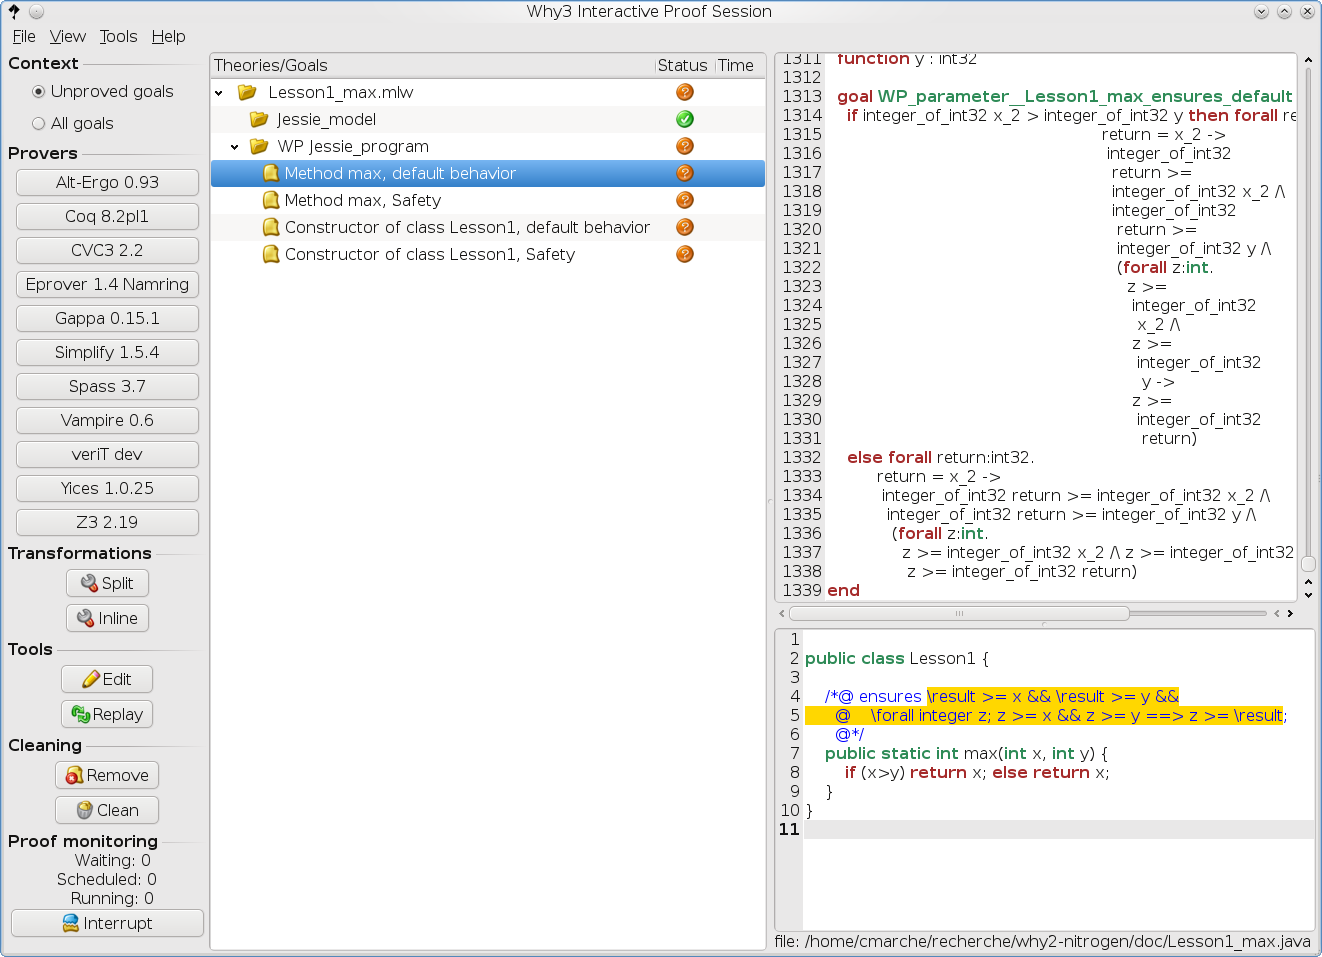
\includegraphics[width=1.2\textwidth]{Lesson1_max_why3_1.png}
  \end{center}
  \caption{Verification conditions displayed in Why3 IDE}
\label{fig:gwhy}
\hrulefill
\end{figure}

  Please refer to Why3's user manual for details on the use of this
  interface. We only remind here the main features.

  The column on the left is a tool bar.  The large window in the
  middle is the tree view of all generated VCs. There are 4 VCs
  generated from this program, given as sub-rows of the row called
  ``WP Jessie program''. Generally speaking, there is one VCs for each
  behavior of each method or constructor. Safety is one of these
  behaviors, which includes checking absence of null dereferencing,
  absence of out-of-bounds array acces, absence of division by zero,
  and other kind of possible runtime errors like that.  In this tree
  view, the first VC has been selected was selected, by clicking on
  the corresponding row. The corresponding specification frim the
  source code is shown on the bottom right part: it is here the
  post-condition we gave to method max. The top right part of the
  window displays the logical formula associated to the VC.

  The left toolbar contains a series of buttons for each prover that
  was detected when you run ``why3config --detect''. A given prover
  can be run on a given goal, or a set of goals by selecting the
  wanted part of the tree. In our example, we can select the row ``WP
  Jessie program'' and click e.g on Alt-Ergo. Clicking further on
  other provers like Z3 or CVC3, will run these on the VCs that are
  not yet proved (see Why3 manual for details). The result is
  displayed on Figure~\ref{fig:why3b}.

\begin{figure}[t]
  \begin{center}
    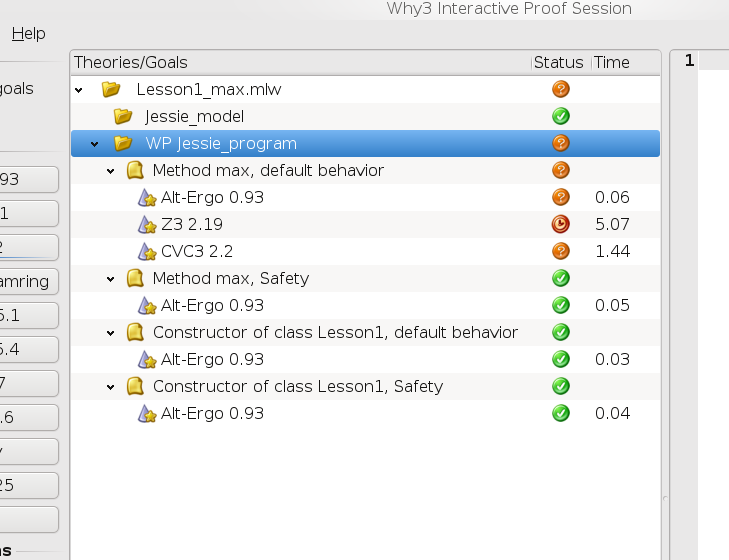
\includegraphics[width=1.0\textwidth]{Lesson1_max_why3_2.png}
  \end{center}
  \caption{Provers run on verification conditions}
\label{fig:why3b}
\hrulefill
\end{figure}

The VC for the post-condition of max is not proved. To investigate
further, and since it is a conjunction of several propositions, it is
a good idea to split it in parts. This is done by selecting the VC and
clicking on the ``split'' button. This results into two subgoals for
that VC. Again, we can click on provers Alt-Ergo, Z3 and CVC3 to check
these subgoals. The second remains unproved. It can be splitted in
parts again, which this time results into 3 subgoals, and provers can
be run again on them. The result is displayed on
Figure~\ref{fig:why3c}.

\clearpage

\begin{figure}[tp]
  \begin{center}
    \hspace*{-0.1\textwidth}
    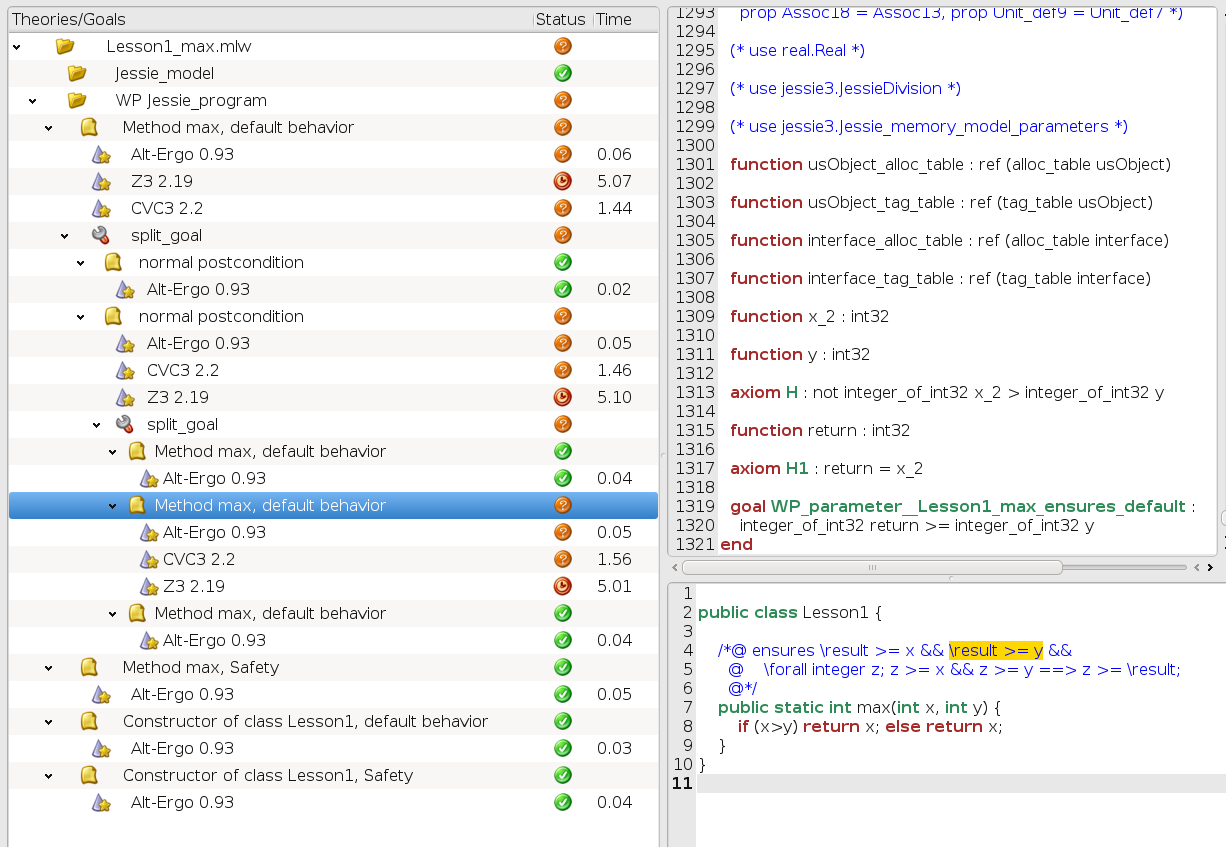
\includegraphics[width=1.2\textwidth]{Lesson1_max_why3_3.png}
  \end{center}
  \caption{Splitting verification condition in parts}
\label{fig:why3c}
\hrulefill
\end{figure}

The subgoal that remains unproved was selected, and the corresponging
spec is shown on the bottom left: it is the part \verb|\result >= y|
which is not valid. Indeed, this comes from our intentional mistake;
the result s not necessarily greater or equal to y in the second
branch.  It is time to fix the source code. You can quit the graphical
interface, and replace with your favorite editor the last \texttt{x}
by \texttt{y}.  If you rerun the \texttt{krakatoa} command as above,
you will see that the state of your proof session was recorded and
thus see all the splitting you made earlier. You notice also that most
of the goals are marked as ``obsolete'' meaning that the results
recorded in your proof sessions are not accurate any more. It is the
right time to use the ``replay'' button of the interface to rerun
prover on all obsolete proofs. Then click on the remaining VC and on a
prover like Alt-ergo, to see that this time the proof is OK. Indeed,
the splittings that you made to reach this state are not necessary
anymore; select the first split and the ``remove'' button, then
restart provers on the first VC, it should be proved. This means that
the method implementation now satisfies its specification.

\clearpage

\section{Loop invariants}
\index{loop invariant}
\index{loop invariant clause@\texttt{loop\_invariant} clause}

Methods get a bit harder to prove in presence of loops. Below is a
contract of a method for computing the square root of an
integer (rounded towards zero).
\input{Lesson1_sqrt.pp}
\index{precondition}
\index{requires clause@\texttt{requires} clause}
The new \texttt{requires} introduce a \texttt{precondition}. This is
formula that is supposed to hold at the beginning of the method call,
here we ask for the parameter \texttt{x} to be non-negative, otherwise
computing its square root would not be possible. The precondition is
not something guaranteed by the method itself: it has to be checked by
the caller of the method.

The \texttt{ensures} clause given states now that (i) the result is
non-negative, (ii) the square of the result is less than or equal to
\texttt{x}, and (iii) the successor of the result has a square which
is greater than \texttt{x}. This ensures that the result is indeed the
square root rounded towards zero.

To implement such a method, we propose an algorithm based on the
following remark: we know that
\[
\sum_{i=0}^{k-1} 2i+1 = k^2
\]
so the square root of $n$ is the smallest integer $k$ such that
\[
\sum_{i=0}^{k} 2i+1
\]
is greater than $n$.

Now, add the following to your class \texttt{Lesson1}.
\input{Lesson1_sqrtbody.pp}
If you generate the VCs now, using
\begin{verbatim}
krakatoa Lesson1.java
\end{verbatim}
you will see the VC for the post-condition, as shown on
Figure~\ref{fig:sqrt} is unproved. (Please ignore the VC ``Safety''
for the moment.)

\begin{figure}[t]
  \begin{center}
    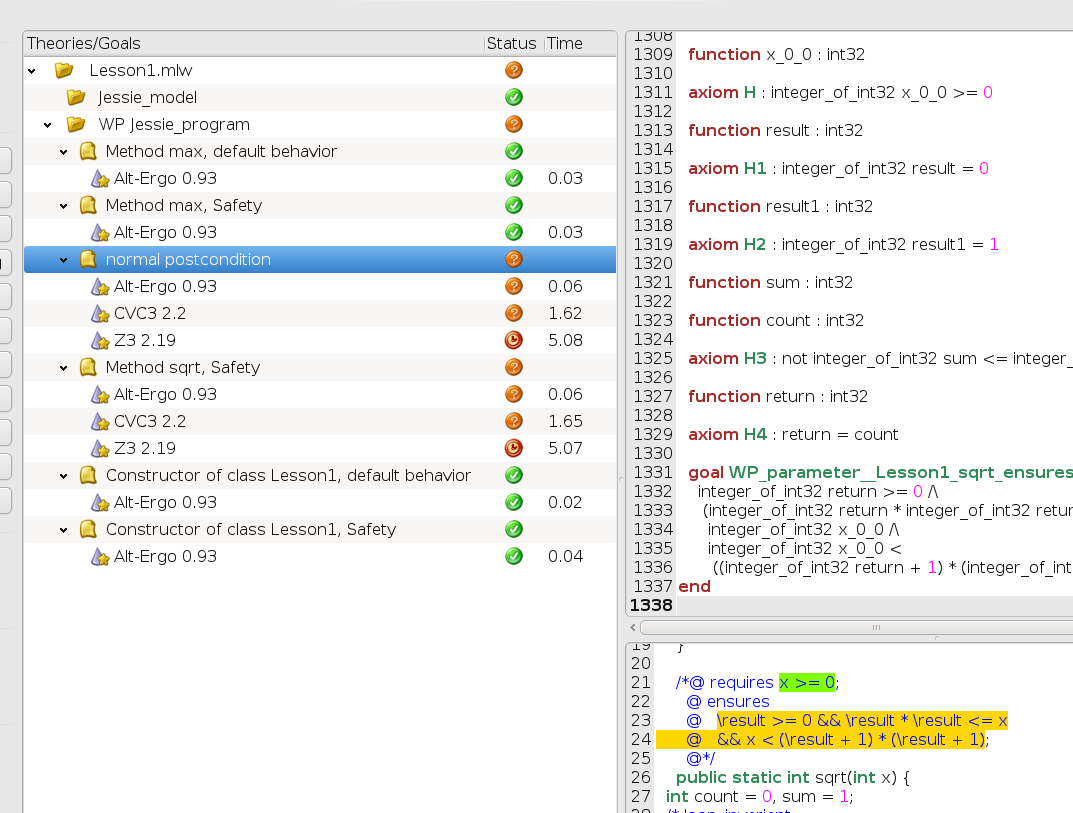
\includegraphics[width=\textwidth]{Lesson1_isqrt_why3_1.png}
  \end{center}
  \caption{Verification conditions for \texttt{sqrt}}
\label{fig:sqrt}
\hrulefill
\end{figure}


Indeed, as usual in Floyd-Hoare logic, to prove a program with a loop
it is required to add a loop invariant to have enough
information.
%More specifically to \Krakatoa{}, you also need to add a
%loop \emph{variant}\index{variant}, an integer expression whose value
%decreases at each loop.
%In that particular example, the variant is not difficult to find: the
%value of \texttt{sum} increases at each loop, until it reaches the
%value of \texttt{x}: so \texttt{x-sum} is a good variant.
Finding the right invariant is usually hard, and usually follows from the
principle of the algorithm. Here, \texttt{count} will increase one by
one, whereas \texttt{sum} will always be the sum of odd integers
between \texttt{1} and \texttt{2*count+1}, that is
\texttt{(count+1)*(count+1)}. So we suggest the following
\input{Lesson1_sqrtloopinv.pp}

If you rerun the krakatoa tool, you should now see that CVC3 and Z3 are able to prove the normal behevior of the method.
% If you rerun the krakatoa tool, run the provers and split the unproved VCs as much as possible, you will see that the subgoal which amounts to show that the property \texttt{sum == count
%   * count} is preserved by the loop, is not proved by any provers. It
% does not mean it is not true: in that case, it illustrates the
% incompleteness of the method, since checking validity of first-order
% formulas is undecidable. Showing that \texttt{sum == count * count} is
% preserver by a loop iteration means to prove that assuming \texttt{sum
%   == count * count} then \texttt{sum'
%   == count' * count'} if  \texttt{count' == count+1}  (instruction
% \texttt{count++}) and \texttt{sum' == sum + 2*count' + 1}. Proving this
% requires to simplify the formulas by applying property of
% distributivity of multiplication over addition. It appears that
% automatic provers are usually quite dumb with multiplication. To help
% them, it is possible to introduce \emph{lemmas} as hints. This is done
% as follows:
% \input{Lesson1_lemmas.pp}
% \index{lemmas}
% \index{lemma declaration@\texttt{lemma} declaration}

% \begin{figure}[t]
%   \begin{center}
%     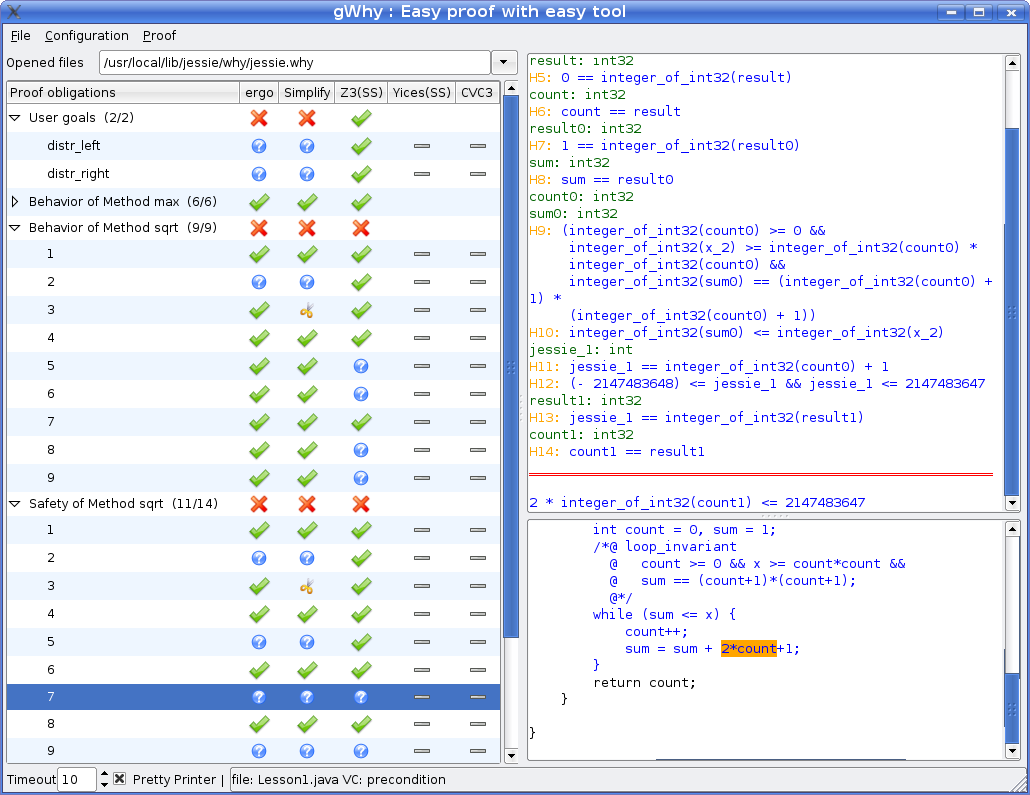
\includegraphics[width=\textwidth]{Lesson1_sqrt2.png}
%   \end{center}
%   \caption{Loop invariant VCs for \texttt{sqrt}}
% \label{fig:sqrt2}
% \hrulefill
% \end{figure}

% Rerunning again krakatoa and the provers results in
% Figure~\ref{fig:sqrt2}. No prover is able to prove every VCs, but
% combining results of the three provers, each VCs is proved.

\subsection*{Safety}
\index{safety}
\index{arithmetic overflow}

\begin{figure}[t]
  \begin{center}
    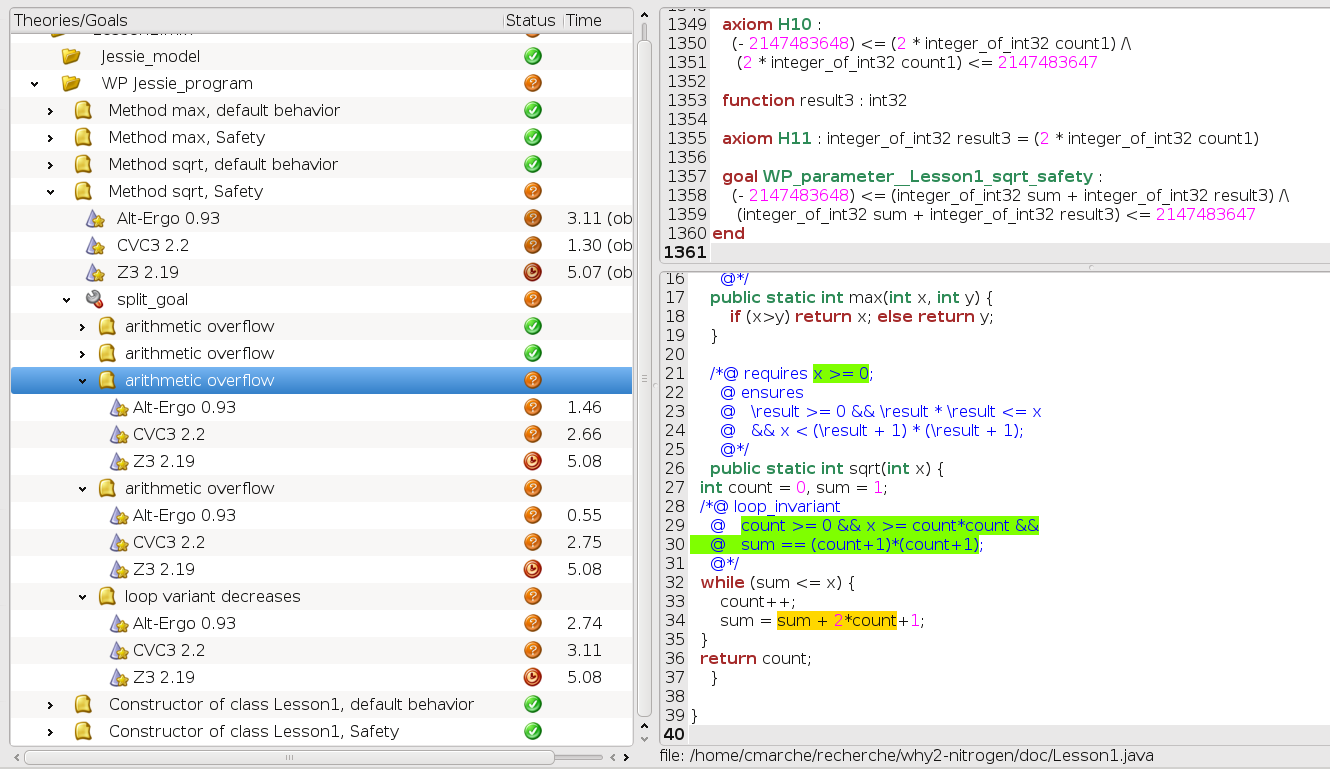
\includegraphics[width=\textwidth]{Lesson1_isqrt_why3_2.png}
  \end{center}
  \caption{Safety VCs for \texttt{sqrt}}
\label{fig:sqrt2}
\hrulefill
\end{figure}

Let's now look at the ``Safety'' section of VCs. This section contains
VCs for checking that no runtime error may occur during
execution. These includes:
\begin{itemize}
\item Division by zero
\item Arithmetic Overflow
\item Null pointer dereferencing
\item Out-of-bounds array access
\end{itemize}

To understand why safety is not proved, let's first split the goal and
try provers on sub-goals. On this example, arithmetic overflow is the
concern. On Figure~\ref{fig:sqrt2}, the focus is put on the VC
corresponding to expression \texttt{sum+2*count} in the source code
(bottom right windows). Looking at the top right window, the goal to prove, which is
\begin{verbatim}
(- 2147483648) <= (integer_of_int32 sum + integer_of_int32 result3)
               <= 2147483647
\end{verbatim}
The constant 2147483648 is $2^{31}$. This goal
amounts to prove that the mathematical result of \texttt{sum + 2*count} fits
into the \texttt{int} type. Indeed it is not
provable, because it is not always true: if the value of $x$ is too
large, arithmetic overflow may occur.

It is possible to find a bound for \texttt{x}, to be added in the
precondition, together with appropriate bounds for \texttt{sum} and
\texttt{count} to be added as loop invariants, to prove the absence of
arithmetic overflow. This is left as an exercise. In some situation,
one may want to simply ignore possible arithmetic overflow. This is
done by added the following \emph{pragma} at the beginning of the
file:
\input{Lesson1_pragma.pp}

You may try this now, and checks that the ``arithmetic overflow'' VCs disappear.

\subsection*{Termination}
\index{termination}
\index{loopvariant clause@\texttt{loop\_variant} clause}

There is another VC that remains to prove, named ``loop variant
decreases''. Indded, since the \texttt{sqrt} method body contains a
\texttt{while} loop, it is possible that the method execution does not
terminate for some of the input. To prove termination, you can add
another clause to the loop annotation: a \texttt{loop\_variant}
clause. An integer expression must follow, which is supposed to
decreases at each loop iteration, and remaining non-negative. On the
\texttt{sqrt} example, that \texttt{x-sum} is decreasing, so you can
add: \input{Lesson1_sqrtdecr.pp}

You can check again that this is proved automatically.

\section{Array accesses}

In this lesson, we now consider arrays. You should now create a new
file \verb|Arrays.java|. Here is the specification of a method for computing
the maximum element of an array of ints, given as argument:
\input{Arrays_findMax.pp}
The precondition is necessary to ensure that \verb|t| is a non-empty
array, so that the maximum exists. An alternative would have been to
raise an exception in that case, but exceptions will be considered
later. We also add the pragma for avoiding arithmetic overflow
checking for simplicity, although in that case there will be no
overflow problem.

We propose the following code for that method:
\input{Arrays_findMaxbody.pp}
The loop invariant ensures that \verb|r| is always the index of the maximum
element of \verb|t| between \verb|0| and \verb|i-1|. We put also as
invariant the facts that \verb|r| and \verb|i| remain in the bounds of
\verb|t|.


\section{Logic predicates}

\index{logic predicates}
\index{predicate declaration@\texttt{predicate} declaration}

The following example is the same is the previous one. We just
introduce a logic predicate to avoid the writing of similar formulas.
See also \url{http://proval.lri.fr/gallery/krakatoa.en.html}.

\input{Arrays_findMax2.pp}


\section{Array updates}

\index{old construct@\bskw{old} construct}
\index{at construct@\bskw{at} construct}

The following method shifts for one cell to the right the contents of
an array. It illustrates the \verb|\old| and the \verb|\at|
constructs.
See also \url{http://proval.lri.fr/gallery/krakatoa.en.html}.

\input{Arrays_shift.pp}

\section{Objects and constructors}

It is time to consider true \Java{} objects. Let's consider the
following class that implements a very simple electronic purse.
See also \url{http://proval.lri.fr/gallery/krakatoa.en.html}.
\input{Purse0.pp}


\section{Calling subprograms, \texttt{assigns} clauses}

See also \url{http://proval.lri.fr/gallery/krakatoa.en.html}.

\index{assigns clause@\texttt{assigns} clause}

\input{Purse_test1.pp}
\input{Purse_test2.pp}

These tests cannot be proved, the \texttt{credit} and
\texttt{withdraw} methods must be given \texttt{assigns} clauses as
follows:
\input{Purse2.pp}

\section{Programs with exceptions}

See also \url{http://proval.lri.fr/gallery/krakatoa.en.html}.

\index{behavior}
\index{behavior declaration@\texttt{behavior} declaration}
\index{signals clause@\texttt{signals} clause}

\input{Purse_withdraw2.pp}

\section{The Dutch National Flag problem}

See also \url{http://proval.lri.fr/gallery/krakatoa.en.html}.

\input{Flag.pp}

\section{Ghost variables}

\index{ghost variables}
\index{ghost declaration@\texttt{ghost} declaration}

The following example illustrates code instrumentation using ghost
variables.
See also \url{http://proval.lri.fr/gallery/krakatoa.en.html}.

\input{Gcd.pp}

\chapter{Specification Language: Reference}
\label{chap:reference}

This chapter is the reference for the specification language. It is
unfortunately largely incomplete, but for missing parts and
explanations we refer to the ACSL Reference
Manual~\cite{baudin09acsl}, which is very close.


\section{Logic expressions}
\label{sec:expressions}

We present the language of expressions one can use in
annotations. These are called \emph{logic expressions}.

This language is essentially the standard multi-sorted first-order
logic. It is a two-valued logic language, made of \emph{propositions}
with standard first-order connectives, built upon a language
of atoms called \emph{terms}.

As far as possible, the syntax of Java expressions is reused:
conjunction is denoted as \verb|&&|, disjunction as \verb+||+ and
negation as \verb|!|.  Additional connectives are \verb|==>| for
implication, \verb|<==>| for equivalence. Universal quantification is
denoted by $\bskw{forall} \tau~x_1,\ldots,\tau~x_n; e$ and existential
quantification by $\bskw{exists} \tau~x_1,\ldots,\tau~x_n; e$.

Terms are built on
\begin{itemize}
\item integer and real arithmetic
\item Java array access and field access
\item Java cast
\item user-defined logic types, and user-defined predicate and logic
  functions, described in Section~\ref{sec:logicspec}
\end{itemize}
In essence, terms correspond to pure Java expressions, with additional
constructs that we will introduce progressively, except that method
and constructor calls are not allowed.

Figure~\ref{fig:gram:lexpr} presents the grammar for the basic
construction of logic expressions.

\begin{figure}[p]
  \fbox{\begin{minipage}{0.97\textwidth} %%%%%%%%%%%%%%%%%%%%%%%%%%%%%%%%%%%%%%%%%%%%%%%%%%%%%%%%%%%%%%%%%%%%%%%%%%
%                                                                        %
%  The Why platform for program certification                            %
%  Copyright (C) 2002-2008                                               %
%    Romain BARDOU                                                       %
%    Jean-Fran�ois COUCHOT                                               %
%    Mehdi DOGGUY                                                        %
%    Jean-Christophe FILLI�TRE                                           %
%    Thierry HUBERT                                                      %
%    Claude MARCH�                                                       %
%    Yannick MOY                                                         %
%    Christine PAULIN                                                    %
%    Yann R�GIS-GIANAS                                                   %
%    Nicolas ROUSSET                                                     %
%    Xavier URBAIN                                                       %
%                                                                        %
%  This software is free software; you can redistribute it and/or        %
%  modify it under the terms of the GNU Library General Public           %
%  License version 2, with the special exception on linking              %
%  described in file LICENSE.                                            %
%                                                                        %
%  This software is distributed in the hope that it will be useful,      %
%  but WITHOUT ANY WARRANTY; without even the implied warranty of        %
%  MERCHANTABILITY or FITNESS FOR A PARTICULAR PURPOSE.                  %
%                                                                        %
%%%%%%%%%%%%%%%%%%%%%%%%%%%%%%%%%%%%%%%%%%%%%%%%%%%%%%%%%%%%%%%%%%%%%%%%%%

%       | "\let" id "=" lexpr ";" lexpr ; local binding
%       | id ":" lexpr ; syntactic naming

\begin{syntax}
  rel-op ::= "==" | "!=" | "<=" | ">=" | ">" | "<"
       \
  bin-op ::= "+" | "-" | "*" | "/" | "%" ;
       | "&&" | "||" |   ; boolean operations
       | "&" | "|" ; bitwise operations
       | "==>" ; boolean implication
       | "<==>" ; boolean equivalence
       \
  unary-op ::= "+" | "-" ; unary plus and minus
       | "!" ; boolean negation
       | "~" ;  bitwise complementation
       \
  lexpr ::= "true" | "false" ;
       | integer ; integer constants
       | real ; real constants
       | id ; variables
       | unary-op lexpr ;
       | lexpr bin-op lexpr ;
       | lexpr (rel-op lexpr)+ ; comparisons, see remark below
       | lexpr "[" lexpr "]" ; array access
       | lexpr "." id  ; object field access
       | "(" type-expr ")" lexpr  ; cast
       | id "(" lexpr ("," lexpr)* ")" ; function application
       | "(" lexpr ")" ; parentheses
       | lexpr "?" lexpr ":" lexpr ;
       | "\forall" binders ";" lexpr ; universal quantification
       | "\exists" binders ";" lexpr ; existential quantification
       \
  binders ::= type-expr variable-ident+ ;
  ("," variable-ident+)*
  \
  type-expr ::= logic-type-expr | Java-type-expr
  \
  logic-type-expr ::= built-in-logic-type ;
  | id ; logic type identifier
  \
  built-in-logic-type ::= "integer" | "real" 
  \
  variable-ident ::= id 
  | variable-ident "[]"
\end{syntax}

%%% Local Variables:
%%% mode: latex
%%% TeX-master: "main"
%%% End:

    \end{minipage}}
  \caption{Grammar of logic expressions}
\label{fig:gram:lexpr}
\end{figure}

Basic additional constructs are as follows:
\begin{description}
% \item[Local binding] $\bskw{let} x = e_1 ; e_2$
%   introduces the name $x$ for
%   expression $e_1$ which can be used in expression $e_2$.

\item[Conditional] $c ? e_1 : e_2$. There is a subtlety
  here: the condition may be either a boolean term or a proposition.  In
  case of a proposition, the two branches must be also proposition, so
  that this construct acts as a connective with the following
  semantics: $ c ? e_1 : e_2$ is equivalent to $(c
  \verb|==>| e_1) \verb|&&| (\verb|!| c \verb|==>| e_2)$

% \item[Syntactic naming] $id \verb|:| e$ is a term or a proposition
%   equivalent to $e$. It is different from local naming with $\bskw{let}$:
%   the name cannot be reused in other terms or proposition. It is only
%   for readability purposes.

\item[Consecutive comparison operators] the construct $t_1~relop_1~t_2~relop_2~t_3 \cdots t_k$ with
  several consecutive comparison operators is a shortcut for
  $t_1~relop_1~t_2 ~\verb|&&|~ t_2~relop_2~t_3 ~\verb|&&|~ \cdots $.
  Nevertheless, it is required that the $relop_i$ operators must be in
  the same ``direction'', \emph{i.e.} they must all belong either to
  $\{\verb|<|, \verb|<=|, \verb|==|\}$ or to
  $\{\verb|>|,\verb|>=|,\verb|==|\}$. For example, expressions
  \verb|x < y > z| and \verb|x != y != z| are forbidden.

\end{description}

\subsection{Operator precedence}

The precedence of Java operators is conservatively extended with
additional operators, as shown Figure~\ref{fig:precedence}. In this
table, operators are sorted from highest to lowest priority. Operators
of same priority are presented on the same line.


\begin{figure}[t]
  \begin{center}
    \begin{tabular}{|l|l|l|}
      \hline
      class 	& associativity & operators \\
      \hline
      selection & left & $\verb|[|\cdots\verb|]|$ \verb|.| \\
      unary 	& right & \verb|!| \verb|~| \verb|+| \verb|-| (cast) \\
      multiplicative & left & \verb|*| \verb|/|  \verb|%| \\
      additive & left & \verb|+| \verb|-| \\
      shift 	& left & \verb|<<| \verb|>>| \verb|>>>| \\
      comparison & left & \verb|<| \verb|<=| \verb|>| \verb|>=| \\
      comparison & left & \verb|==| \verb|!=| \\
      bitwise and & left & \verb|&| \\
      bitwise xor & left & \verb|^| \\
      bitwise or & left & \verb+|+ \\
      connective and     & left & \verb|&&| \\
      connective xor & left & \verb+^^+ \\
      connective or & left & \verb+||+ \\
      connective implies & right & \verb|==>| \\
      connective equiv & left & \verb|<==>| \\
      ternary connective & right & $\cdots\verb|?|\cdots\verb|:|\cdots$ \\
      binding & left & \bskw{forall} \bskw{exists} %\bskw{let}
      \\
%      naming & right & \verb|:| \\
      \hline
    \end{tabular}
  \end{center}
  \caption{Operator precedence}
\label{fig:precedence}
\end{figure}

% There is an additional ambiguity between the connective
% \verb|..?..:..| and the naming with \verb|:|. For example, in the
% expression \verb|x?y:z:t|, the precedence table does not enforce
% whether this should be seen as \verb|x?(y:z):t| or \verb|x?y:(z:t)|.
% Such a case must considered as a syntax error, and should be fixed
% by explicitly using parentheses.

\subsection{Semantics}
\label{sec:twovaluedlogic}

The semantics of logic expressions is based on
mathematical first-order
logic~(\url{http://en.wikipedia.org/wiki/First_order_logic}), thus it
is a 2-valued logic with only total functions. Consequently,
expressions are never ``undefined''.

This design choice has to be emphasized because it is not
straightforward, and specification writer should be aware of that. The
issues are shared with JML. A comprehensive list of issues has been
compiled by Patrice Chalin~\cite{chalin05ftfjp,chalin07icse}.

The choice of having only total functions allows to write for example
the term \verb|1/0|, or \verb|p.f| when p is null, or \verb|t[n]|
where n is outside the array bounds. In
particular, the predicates
\begin{eqnarray*}
  1/0 &\verb|==|& 1/0 \\\relax
  p.f &\verb|==|& p.f
\end{eqnarray*}
are true, since they are instances of the general axiom $\forall x,
x\verb|==|x$ of first-order logic.

So, it is up to the writer of specification to take care of writing
consistent assertions.

\subsection{Typing}

The language of logic expressions is typed (as for \emph{multi-sorted}
first-order logic). Types are either Java types or \emph{logic types}
defined as follows:
\begin{itemize}
\item ``Mathematical'' types: \verb|integer| for unbounded,
  mathematical integers; \verb|real| for real numbers.
%, \verb|boolean|
%  for booleans (with values written as \verb|\true| and \verb|\false|).
\item Logic types introduced by specification writer (see
  Section~\ref{sec:logicspec}).
\end{itemize}
There are implicit coercions for numeric types:
\begin{itemize}
\item integer types \verb|char|, \verb|byte|, \verb|short|, \verb|int| and
  \verb|long| are all subtypes of type \verb|integer|,
\item \verb|integer| is itself a subtype of type \verb|real|,
\item types \verb|float| and \verb|double| are subtypes of type \verb|real|.
\end{itemize}
Notes:
\begin{itemize}
\item There is a distinction between booleans and propositions. An
  expression like $x<y$, in a term position returns a boolean, and is
  also allowed in a proposition position.
\item Quantification can be made over any type: logic types and any Java
  types. Quantification over objects must be carefully designed,
  regarding the memory state where field accesses are done: see
  Section~\ref{sec:quantification} and
  Section~\ref{sec:logicalstates}.
\end{itemize}

% Formal typing rules for terms are given in appendix~\ref{sec:typingrules}

\subsection{Integer arithmetic and machine integers}

The following integer arithmetic operations apply to
\emph{mathematical integers}: addition, subtraction, multiplication,
unary minus, division and modulo. The value of a Java variable of an
integer type is promoted to a mathematical integer. As a consequence,
there is no such thing as ``overflow'' in logic expressions.

For division and modulo, the results are not specified if divisor is
zero, otherwise if $q$ and $r$ are the quotient and the remainder of
$n$ divided by $d$ then:
\begin{itemize}
\item $|d.q| \leq |n|$, and $|q|$ is maximal for this property ;
\item $q$ is zero if $|n|<|d|$ ;
\item $q$ is positive if $|n|\geq|d|$ and $n$ and $d$ have the same sign ;
\item $q$ is negative if $|n|\geq|d|$ and $n$ and $d$ have the opposite signs ;
\item $q.d+r = n$ ;
\item $|r|<|d|$ ;
\item $r$ is zero or has the same sign as $d$.
\end{itemize}

\begin{example}
  The following examples illustrates the results of division and modulo depending on signs of arguments:
  \begin{itemize}
  \item \verb|5/3| is 1 and \verb|5%3| is 2
  \item \verb|(-5)/3| is -1 and \verb|(-5)%3| is -2
  \item \verb|5/(-3)| is -1 and \verb|5%(-3)| is 2
  \item \verb|(-5)/(-3)| is 1 and \verb|(-5)%(-3)| is -2
  \end{itemize}
\end{example}

\subsubsection{Hexadecimal and octal constants}

Hexadecimal and octal constants always denote non-negative integers.

\subsubsection{Casts and overflow}

In logic expressions, casting operations from mathematical integers
towards a Java integer type $t$ (among \texttt{char}, \texttt{byte},
\texttt{short}, \texttt{int} and \texttt{long}) is
allowed, and is interpreted as follows: the result is the unique value
of the corresponding type that is congruent to the mathematical result
modulo the cardinal of this type.
\begin{example}
  \texttt{(byte)1000} is $1000 \bmod 256$ \emph{i.e.} $-24$.
\end{example}

If one wants to express, in the logic, the result of the Java
computations of an expression, one should add all necessary casts. For
example, the logic expression which denotes the result of Java
computation of $x*y+z$ is \texttt{(int)((int)(x*y)+z)}.

% TODO Si la conjecture suivante est vraie, alors il
%   faudrait en parler: Si e1 et e2 sont des expressions d'un type
%   entier de C, quels qu'ils soient et si op est une operation binaire
%   sur entiers, alors l'operation C $e1~op~e2$ (de type $\tau$),donne
%   le meme resultat que l'expression logique $(\tau)(e_1~op~e_2)$ ou
%   $op$ est l'operation logique sur $Z$. Ce cast permet donc a
%   l'utilisateur de parler du resultat du calcul C d'une expressions
%   dans la logique


Remark: implicit casts from integers to Java integer type are forbidden.
%input{integer-cast.pp}



\subsubsection{Quantification}
\label{sec:quantification}

Quantification can be either on mathematical \verb|integer| or bounded
types \verb|short|, \verb|char|, etc. In the latter case,
quantification corresponds to integer quantification over the
corresponding interval.
\begin{example}
The formula
  \begin{center}
    \verb|\forall byte b; b <= 1000|
  \end{center}
is valid since it is equivalent to
\begin{center}
  \verb|\forall integer b; -128 <= b <= 127 ==> b <= 1000|
\end{center}
\end{example}

\subsubsection{Bitwise operations}

Like arithmetic operations, bitwise operations apply to any
mathematical integers: any mathematical integer as a unique infinite
2-complement binary representation with infinitely many 0 (for
non-negative numbers) or 1 (for negative numbers) on the left. Then
bitwise operations apply to these representation.
\begin{example}
  \begin{itemize}
  \item \verb|7 & 12| = $\cdots 00111 \verb|&| \cdots 001100$ =
    $\cdots 00100$ = 4
  \item \verb+-8 | 5+ = $\cdots 11000 \verb+|+ \cdots 00101$ = $\cdots
    11101$ = -3
  \item \verb+~5+ = $\verb|~|\cdots 00101$ = $\cdots 111010$ = -6
  \item \verb+-5 << 2+ = $\cdots 11011 \verb|<<| 2$ = $\cdots
    11101100$ = -20
  \item \verb+5 >> 2+ = $\cdots 00101 \verb|>>| 2$ = $\cdots 0001$ = 1
  \item \verb+-5 >> 2+ = $\cdots 11011 \verb|>>| 2$ = $\cdots 1110$ =
    -2
  \end{itemize}
\end{example}

\subsection{Real numbers and floating point numbers}

Floating-point constants and operations are interpreted as
mathematical real numbers. A Java variable of type float or double is
implicitly promoted to a real. Integers are promoted to reals if necessary.
\begin{example}
$2 * 3.5$ denotes the real number 7
\end{example}
Comparisons operators are interpreted as real operators too.

% TODO  syntaxe pour abs et power ? a priori non, on peut
%   fournir une library pour les reels avec abs(), power(), mais
%   proposer des syntaxes speciales parait difficile

%   mais: on pourrait permettre des definition d'operateurs infixes


% \subsubsection{Casts, infinity and NaNs}

% Casting from an integer type or a float type to a float or a double is
% as in Java: same conversion operations applies.

% Casting a real number $x$ to a float (resp. a double) results in a
% float value $y$ with the nearest-even rounding mode (see IEEE 754
% norm), which is the closest to $x$ real number which is representable
% in the float (resp. double) type. If the source real number is too
% large, this may also result into one of the special values +infinity
% and -infinity. This semantics ensures that the float result of a Java
% operation $e_1 op e_2$ on floats, if the default rounding mode is not
% changed in the program, might be obtained in the logic under the form
% $(float)(e_1 op e_2)$.

% \begin{example}
%   We have
%   \verb|(float)0.1| = $13421773 \times 2 ^{-27}$ which is equal to
%   $0.10000000149006473916$
% \end{example}

% Rounding of real number towards a float with other rounding modes
% might be obtained via specific logic functions given in external
% libraries. As well, classical mathematical operations like
% exponential, sine, cosine, etc. are supposed to be available in some
% library (see Section~\ref{sec:libreal}).


% \subsubsection{Quantification}

% Quantification over a variable of type \verb|real| is of course usual
% quantification over real numbers.

% Quantification over float (resp. double) types is allowed too, and are
% supposed to range over all real numbers representable as floats (resp
% doubles). In particular, this does not include NaN, +infinity and
% -infinity in the considered range.

\section{Simple contracts}


A simple contract is an annotation that can be given to constructors
and methods (not depending on whether they are given a body or are
abstract). It is a contract between the caller and the callee, made of
a precondition and a postcondition:
\begin{itemize}
\item Precondition:
  \begin{itemize}
  \item The caller is responsible for ensuring it before call
  \item The callee assumes it at entrance of its body
  \end{itemize}
\item Postcondition:
  \begin{itemize}
  \item The callee must guarantee it at normal exit
  \item The caller can then assume it after the call
  \end{itemize}
\end{itemize}
Additionally, a contract can be completed with a \emph{frame clause}
which describes side-effects, and acts as a postcondition.

Note that post-conditions of simple contracts only concern normal
exit: exiting with exceptions can be specified using additional
\emph{behavior clauses} described in Section~\ref{sec:behaviors}

\begin{figure}[t]
  \fbox{\begin{minipage}{0.97\textwidth}
      %%%%%%%%%%%%%%%%%%%%%%%%%%%%%%%%%%%%%%%%%%%%%%%%%%%%%%%%%%%%%%%%%%%%%%%%%%
%                                                                        %
%  The Why platform for program certification                            %
%  Copyright (C) 2002-2008                                               %
%    Romain BARDOU                                                       %
%    Jean-Fran�ois COUCHOT                                               %
%    Mehdi DOGGUY                                                        %
%    Jean-Christophe FILLI�TRE                                           %
%    Thierry HUBERT                                                      %
%    Claude MARCH�                                                       %
%    Yannick MOY                                                         %
%    Christine PAULIN                                                    %
%    Yann R�GIS-GIANAS                                                   %
%    Nicolas ROUSSET                                                     %
%    Xavier URBAIN                                                       %
%                                                                        %
%  This software is free software; you can redistribute it and/or        %
%  modify it under the terms of the GNU General Public                   %
%  License version 2, as published by the Free Software Foundation.      %
%                                                                        %
%  This software is distributed in the hope that it will be useful,      %
%  but WITHOUT ANY WARRANTY; without even the implied warranty of        %
%  MERCHANTABILITY or FITNESS FOR A PARTICULAR PURPOSE.                  %
%                                                                        %
%  See the GNU General Public License version 2 for more details         %
%  (enclosed in the file GPL).                                           %
%                                                                        %
%%%%%%%%%%%%%%%%%%%%%%%%%%%%%%%%%%%%%%%%%%%%%%%%%%%%%%%%%%%%%%%%%%%%%%%%%%

\begin{syntax}
  contract ::= (requires-clause | assigns-clause |
  ensures-clause ) *
  \
  requires-clause ::= "requires" proposition ";"
  \
  assigns-clause ::= "assigns" locations ";"
  \
  locations ::= location ("," location) * | "\nothing"
  \
  ensures-clause ::= "ensures" proposition ";"
\end{syntax}

    \end{minipage}}
    \caption{Grammar of simple contracts}
  \label{fig:gram:contracts}
\end{figure}

The syntax of simple contracts syntax is given
Figure~\ref{fig:gram:contracts}. Let's consider a simple contract of the following
generic form:
\begin{flushleft}\ttfamily
/*@ requires $P_1$; \\
~~@ requires $P_2$; \\
~~@ assigns $L_1$; \\
~~@ assigns $L_2$; \\
~~@ ensures $E_1$; \\
~~@ ensures $E_2$; \\
~~@*/
\end{flushleft}
the semantics of such a contract can be rephrased as follows:
\begin{itemize}
\item The caller must guarantee that the callee is called in a
  state (called \emph{prestate})  where the property $P_1 \verb|&&| P_2$ holds.
\item When the callee returns normally, the property
  $E_1 \verb|&&| E_2$ must hold in the corresponding \emph{poststate}.
\item All memory locations of the prestate that do not belong to the
  set $L_1 \cup L_2$ remain allocated and are left unchanged in the
  poststate.
\end{itemize}
Thus, the contract above is equivalent to the following
simplified one:
\begin{flushleft}\ttfamily
/*@ requires $P_1 \verb|&&| P_2$; \\
~~@ assigns $L_1,L_2$; \\
~~@ ensures $E_1 \verb|&&| E_2$; \\
~~@*/
\end{flushleft}
The multiplicity of clauses are proposed mainly to improve
readibility. Also, if no clause \bkw{requires} is given, it defaults
to requiring `true', and similarly for \bkw{ensures} clause. Giving no
\bkw{assigns} clause means that side-effects are not specified: it
potentially modifies everything.


\section{Behavior clauses}
\label{sec:behaviors}

A simple contract can be augmented with \emph{behaviors}.


A normal behavior clause as the form
\begin{flushleft}\ttfamily\upshape\parindent 0pt
\begin{slshape}\color{blue}\textbf{behavior}~\textsl{id}~:~\\
~~\textbf{assumes}~\textsl{A}~;~\\
~~\textbf{assigns}~\textsl{L}~;~\\
~~\textbf{ensures}~\textsl{E}~;~\end{slshape}
\end{flushleft}
The semantics of such a behavior is as follows. The callee guarantees
that if it returns normally, then in the post-state:
\begin{itemize}
\item $\bskw{old}(A) \Rightarrow E$ holds
\item If $\bskw{old}(A)$ holds, each location of the pre-state not
  in $L$ remains allocated and unchanged in
  the post-state
\end{itemize}

An exceptional behavior clause as the form
\begin{flushleft}\ttfamily\upshape\parindent 0pt
\begin{slshape}\color{blue}\textbf{behavior}~\textsl{id}~:~\\
~~\textbf{assumes}~\textsl{A}~;~\\
~~\textbf{assigns}~\textsl{L}~;~\\
~~\textbf{signals}~(\textsl{Exc})~\textsl{E}~;~\end{slshape}
\end{flushleft}
The semantics of such a behavior is as follows. The callee guarantees
that if it exits with exception Exc, then in the post-state:
\begin{itemize}
\item $\bskw{old}(A) \Rightarrow E$ holds
\item If $\bskw{old}(A)$ holds, each location of the pre-state not
  in $L$ remains allocated and unchanged in
  the post-state
\end{itemize}
Notice that in $E$, \bskw{result} is bound to the exception object thrown.


\section{Code annotations}

\subsection{Assertions}

  \begin{itemize}
  \item Additional clause:
    \begin{flushleft}\ttfamily\color{blue}
      //@ assert \textsl{prop}
    \end{flushleft}
  specify that the given property is true at the corresponding
    program point
%   \item Assertions can be associated to behaviors, as:
%     \begin{flushleft}\ttfamily\color{blue}
%       //@ for $b_1,\ldots,b_n$: assert \textsl{prop}
%    \end{flushleft}

  \end{itemize}

\subsection{Loop annotations}

  \begin{itemize}
  \item Additional clause for loops:
    \begin{flushleft}\ttfamily\color{blue}
      /*@ loop\_invariant \textsl{prop} \\
      ~~@ loop\_assigns \textsl{tset} \\
      ~~@*/
    \end{flushleft}
    specify that
    \begin{itemize}
    \item the given property is an inductive loop invariant for the
      loop:
      \begin{itemize}
      \item true at loop entrance
      \item preserved by loop body
      \end{itemize}
    \item side-effect of the loop are included in the given tset
    \end{itemize}
%  \item Can be associated to behaviors too
  \end{itemize}

% \subsection{Statement contracts}

%   \begin{itemize}
%   \item Same as function contracts, associated to statements
%   \item Acts as embedding the corresponding statement in a black box,
%     as if it was a function call
%   \item May have additional clauses in behaviors, to be used in place
%     of the throws clause:
%     \begin{flushleft}\ttfamily\color{blue}
%       /*@ breaks \textsl{prop} \\
%       ~~@ continues \textsl{prop} \\
%       ~~@ returns \textsl{prop} \\
%       ~~@*/
%     \end{flushleft}
%     to deal with corresponding abrupt termination

%   \item Can be associated to behaviors too
%   \end{itemize}


% \subsection{Code Invariants}

%   \begin{itemize}
%   \item Purpose: support for arbitrary \texttt{goto}s
%   \item Similar to assertions, but acts as inductive properties like
%     loop invariants.
%   \item Inductive scheme is guided by the control flow graph
%     \cite{Filliatre07mix}
%   \end{itemize}



\section{Data invariants}


  A class invariant is a property attached to a class. This property
  is supposed to hold on any object of that class. More precisely, it
  holds at method entrance and exit, and at the exit of constructor.
%  satisfy ata supposed to hold ``permanently''.

%   An invariant may be either
%   \begin{itemize}
%   \item a \emph{global} invariant: on global variables
%   \item or a \emph{type} invariant: apply on any variable of this type.
%   \end{itemize}
%   Independently, it can be either
%   \begin{itemize}
%   \item a \emph{strong} invariant: true at execution step
%   \item a \emph{weak} invariant: true at function boundaries
%   \end{itemize}



\section{Advanced modeling language}
\label{sec:logicspec}

\subsection{Logic definitions}

  \begin{itemize}
  \item New logic functions and predicates can be defined
%  input{.pp}
%  \item Arbitrary recursion is allowed
%  input{fib.c.pp}
  \end{itemize}

\subsection{Hybrid predicates}
\label{sec:logicalstates}

  \begin{itemize}
  \item Logic functions and predicates may depend on memory heap
  \item In such a case, logic labels are required:
%    input{max\_index.c.pp}
  \item Indeed, with only one label, the following is allowed too:
%    input{max\_index2.c.pp}
  \end{itemize}

\subsection{Abstract data types}

  New logic data types (i.e. immutable) can be introduced abstractly
  by giving
  \begin{itemize}
  \item a type name
  \item the profile of logic functions and predicates operating on it
  \item a set of axioms
  \end{itemize}


% \subsection{Concrete data types}

%   \begin{itemize}
%   \item logic types may be defined using
%     \begin{itemize}
%     \item sum types
%     \item record types
%     \end{itemize}
%   \item For sum types: pattern matching
%   \item For record types: $t.f$ notation
%   \item Also built-in: pairs
%   \end{itemize}

% \subsection{Parametric polymorphism}

%   \begin{itemize}
%   \item Parametric polymorphism is proposed, with a C++-like syntax

%   \end{itemize}

% \subsection{Higher-order functions}

%   \begin{itemize}
%   \item The term $\bskw{lambda} ~\textsl{type}~ \textsl{x} ~;~
%     \textsl{t}$
%   stands for the function mapping $x$ to $t$
%   \item Special constructs:
% \begin{eqnarray*}
%     \bskw{max}(i,j,f) &=& \max \{ f(i),f(i+1), \ldots, f(j) \} \\
%     \bskw{min}(i,j,f) &=& \min \{ f(i),f(i+1), \ldots, f(j) \} \\
%     \bskw{sum}(i,j,f) &=& f(i)+f(i+1)+\cdots+f(j) \\
%     \bskw{product}(i,j,f) &=& f(i)\times f(i+1) \times \cdots \times f(j) \\
%     \bskw{numof}(i,j,f) &=& \# \{ k \mid i \leq k \leq j ~\land~ f(k) \} \\
% &=& \bskw{sum}(i,j,\bskw{lambda}~\kw{integer}~k ; \\
% && \hspace*{20mm} f(k) ? 1 : 0)
%   \end{eqnarray*}
%   \end{itemize}

\section{Termination}

\subsection{Loop variants}

  \begin{itemize}
  \item A loop can be annotated with a \emph{variant}: an integer
    expression that decreases at each iteration, using the clause
    \verb|loop_variant|.
%  \item Example:
%    input{bsearchvariant.c.pp}
  \end{itemize}


% \subsection{Recursive functions}

%   \begin{itemize}
%   \item A recursive function can be also annotated with a variant

%     input{fact.c.pp}

%   \item Mutual recursion supported too
%   \end{itemize}

% \subsection{Arbitrary termination order}

%   \begin{itemize}
%   \item Termination order can different from the default
%   \item Order introduced as:
%     \begin{flushleft}\ttfamily\color{blue}
%       //@ predicate $R(\tau x,\tau y)$
%     \end{flushleft}
%   \item Loop variants:
%     \begin{flushleft}\ttfamily\color{blue}
%       //@ loop variant \textsl{term} \kw{for} $R$
%     \end{flushleft}
%   \item Recursive functions:
%     \begin{flushleft}\ttfamily\color{blue}
%       //@ decreases \textsl{term} \kw{for} $R$
%     \end{flushleft}
%   \item For mutual recursion: the same $R$ is required
%   \end{itemize}


\section{Ghost variables}


% \section{Ghost code}

%   \begin{itemize}
%   \item Goal: code instrumentation
%   \item Code is augmented with
%     \begin{itemize}
%     \item global ghost declarations of variables and functions
%     \item In regular function code:
%       \begin{itemize}
%       \item ghost parameters
%       \item local ghost variables
%       \item ghost statements (include ghost \kw{else})
%       \end{itemize}
%     \end{itemize}
%   \item Semantics:
%     \begin{center}\color{red}
%       ghost statements must not change the regular program execution
%     \end{center}
%   \end{itemize}


% \section{Model variables}


\chapter{Appendices}

\section{Requirements}
\label{app:requirements}


Compiling from sources requires Objective Caml
compiler, version 3.09 or higher.

External theorem provers must be installed. See the page~\url{http://why.lri.fr/provers.html}

For using the Coq interactive prover, you need \Coq{} version 8.0 or
higher.

\section{Installation procedure}

\subsection{From the sources}

Get a copy of sources at the web page \url{http://why.lri.fr/}.

Decompress the archive in a directory of your choice.

Run commands
\begin{verbatim}
./configure
make
make install
\end{verbatim}

\subsection{Binaries}

Please look at the web page \url{http://why.lri.fr/} for binaries for
popular architectures. Krakatoa is distributed as part of the Why
debian package, available on standard repositories of debian-based
distributions.

\section{Summary of features and known limitations}
\label{sec:features}

\begin{itemize}
%\item No checking of arithmetic overflow

\item Unsupported kind of statements in translation: ...

\item exception NullPointerException and ArrayOutOfBoundsException are
required NOT to be thrown, and consequently should not be caught.

%\item Method parameters are not modifiable.

% \item For recursive or mutually recursive methods, only partial
% correctness is guaranteed.

%\item some valid Java identifiers should not be used in your programs,
%  unless some name clashes may occur: identifiers starting by
%  \verb|krak| ;
%  names introduced in the generated model: \verb|access|,
%  \verb|update|, etc. ; keywords of \Why: result, parameter, etc.
\end{itemize}

\section{Contacts}

The webpage for Krakatoa is at URL \url{http://krakatoa.lri.fr/} and
the webpage for the Why platform in general is at
\url{http://why.lri.fr}.

For general questions regarding the use of the tool, please use the
Why mailing list. You need to subscribe to the list before sending a
message to it. To subscribe, follow the instructions given on page
\url{http://lists.gforge.inria.fr/cgi-bin/mailman/listinfo/why-discuss}

For bug reports, please use the bug tracking system at
\url{https://gforge.inria.fr/tracker/?atid=4012&group_id=999&func=browse}. For
security reasons, you need to register before submitting a new
bug. Please create an account there, where you can put "ProVal" for
the required field "INRIA Research Project you work with or work in".

In case if the mailing list above is not appropriate, you can contact
the authors directly at the following address: \url{mailto:Claude dot
  Marche at inria dot fr}.

\cleardoublepage

\addcontentsline{toc}{chapter}{\bibname}
\bibliographystyle{plain}
\bibliography{./biblio}
%\input{biblio-demons}
\cleardoublepage

\addcontentsline{toc}{chapter}{\indexname}
\printindex
\cleardoublepage

\end{document}











\section{Loop invariants}
\index{loop invariant}
\index{invariant clause@\texttt{invariant} clause}

Methods get a bit harder to prove in presence of loops. Below is the
specification of a method for computing the square root of an
integer (rounded down).
\input{Lesson1_sqrt.pp}
We propose an algorithm based on the following remark: we know that
\[
\sum_{i=0}^{k-1} 2i+1 = k^2
\]
so the square root of $n$ is the smallest integer $k$ such that
\[
\sum_{i=0}^{k} 2i+1
\]
is greater than $n$.

Please, add the following to your class \texttt{Lesson1}.
\input{Lesson1_sqrtbody.pp}
If you generate the proof obligations now, using
\begin{verbatim}
krakatoa -p tutorial Lesson1.sqrt
make -C tutorial coq
\end{verbatim}
you will realize soon that they are not provable. Indeed, as usual in
Floyd-Hoare logic, it is required to add a loop invariant to have
enough information. More specifically to \Krakatoa{}, you also need to
add a loop \emph{variant}\index{variant}, an integer expression whose
value decreases at each loop.

In that particular example, the variant is not difficult to find: the
value of \texttt{sum} increases at each loop, until it reaches the
value of \texttt{x}: so \texttt{x-sum} is a good variant.

Finding the right invariant is usually hard, and usually follows from the
principle of the algorithm. Here, \texttt{count} will increase one by
one, whereas \texttt{sum} will always be the sum of odd integers
between \texttt{1} and \texttt{2*count+1}, that is
\texttt{(count+1)*(count+1)}. So we suggest the following
\input{Lesson1_sqrtloopinv.pp}
Now let's go to the proof of obligations, for example by running
\begin{verbatim}
coqide Lesson1_sqrt_why.v
\end{verbatim}
The first proof obligation is
required to prove that the loop invariant is true when
entering the loop. It is is automatically solved by the
the \verb|intuition| tactic.
The second proof obligation, after running
the \verb|intuition| tactic, results in two subgoals:
\begin{small}
\begin{verbatim}
x : Z
HW_1 : x >= 0
count : Z
sum : Z
HW_3 : sum <= x
H0 : sum = (count + 1) * (count + 1)
H1 : count >= 0
H2 : x >= count * count
count0 : Z
HW_4 : count0 = count + 1
sum0 : Z
HW_5 : sum0 = sum + 2 * count0 + 1
______________________________________(1/2)
x >= count0 * count0
______________________________________(2/2)
sum0 = (count0 + 1) * (count0 + 1)
\end{verbatim}
\end{small}
These goals are required to prove that the loop invariant remains true
in any execution of the loop body. Think of variables \verb!count! and
\verb!sum! as the values of the corresponding memory cells before the
execution, and
the ones indexed by 1 as the value after the execution.  Notice that
the proof of decrease of the variant has been solved automatically.

Let's solve the first goal: if you replace \verb|count0| by its value
\verb|count+1| given by \verb|HW_4|, you have to prove
\verb|x >= (count+1)*(count+1)|, something that follows immediately from
\verb|HW_3| and \verb|H0| by linear arithmetic. So the tactic
\verb|subst count0; omega.| solves the goal. For the second one, if
you replace \verb|sum0|, \verb|sum| and \verb|count0| by there values
in hypotheses, then the goal becomes a trivial ring equality, so the tactic
\verb|subst sum0 sum count0; ring.| is enough.

% \begin{small}
% \begin{verbatim}
% x : Z
% Pre4 : x >= 0
% sum : Z
% Post5 : sum = 1
% count : Z
% Post4 : count = 0
% ______________________________________(1/2)
% x >= count * count

% ______________________________________(2/2)
% sum = (count + 1) * (count + 1)
% \end{verbatim}
% \end{small}
% these are required to prove that the loop invariant is true when
% entering the loop. Proofs are trivially done by substitution of
% these variables and linear arithmetic:
% \begin{small}
% \begin{verbatim}
% subst count; omega.
% subst count sum; omega.
% \end{verbatim}
% \end{small}

The third and last proof obligation is required to show that the
post-condition of the method is satisfied, provided that the invariant
is true after the loop, and also that the while condition is
false. These are automatically done by the \verb|intuition| tactic.

\section{Array accesses}

In this lesson, we now consider arrays. You should now create a new
file \verb|Arrays.java|. Here is the specification of a method for computing
the maximum element of an array of ints, given as argument:
\input{Arrays_findMax.pp}
The precondition is necessary to ensure that \verb|t| is a non-empty
array, so that the maximum exists. An alternative would have been to
raise an exception in that case, but exceptions will be considered
later.

We propose the following code for that method:
The loop invariant ensures that \verb|r| is always the index of the maximum
element of \verb|t| between \verb|0| and \verb|i-1|. We put also as
invariant the facts that \verb|r| and \verb|i| remain in the bounds of
\verb|t|.

On this method, \Krakatoa{} and then \Why{} produce six proof
obligations. Let's see them in details. The first one is
\begin{small}
\begin{verbatim}
______________________________________(1/1)
forall (t : value) (alloc : alloc_table),
(t <> Null /\ arraylength alloc t >= 1) /\ instanceof alloc t ArrIntType ->
t <> Null /\ is_valid_index alloc t 0
\end{verbatim}
\end{small}
which must be read as follows: given a value \verb|t| and a store
\verb|alloc|, 0 is a valid index for \verb|t| in \verb|alloc|, provided
three conditions: \verb|t| is not null, \verb|t.length >=1|, and
\verb|t| is an instance of \verb|int[]|.

\index{is_valid_index@\texttt{is\_valid\_index}}
\index{instanceof@\texttt{instanceof}}
\index{arraylength@\texttt{arraylength}} \index{store@\texttt{store}}
In the \Coq{} modeling of Java, generated by \Krakatoa{},
\verb|value|\index{value} is the type of any non-primitive Java value,
that is either the \verb|null| value\index{Null@\texttt{Null}}, or an
object or array \emph{reference} (i.e. a memory address). Primitive
values of type \verb|int| or \verb|boolean| are represented by
elements of \verb|Z| or \verb|bool| (floats are not supported yet).

\begin{figure}[t]
\newcommand{\case}{\multicolumn{1}{|r|}{\phantom{0}}}
\begin{center}
\begin{tabular}{c|c|rrrrrrrrrr}
\multicolumn{3}{r}{} & \qquad & \qquad & \qquad & \qquad & \qquad \\
\multicolumn{2}{r}{\texttt{alloc:alloc\_table}} & \multicolumn{1}{r}{} &
\multicolumn{9}{l}{\texttt{intA : int memarray}} \\
\multicolumn{2}{r}{\qquad\qquad} & & \footnotesize 0 & \footnotesize 1 &
\footnotesize 2 & \footnotesize 3 & \multicolumn{4}{l}{$\cdots$} \\
\cline{2-2}\cline{4-8}
$a_1$  & int[5]     & & \case & \case &\case&\case&\case\\
\cline{2-2}\cline{4-11}
$a_2$  & int[8]    & &\case & \case &\case&\case&\case&\case&\case&\case\\
\cline{2-2}\cline{4-11}
$a_3$  & int[3]    & &\case& \case &\case \\
\cline{2-2}\cline{4-6}
$\vdots$  & $\vdots$    & & \multicolumn{2}{l}{$\vdots$}
\end{tabular}
\end{center}
\caption{Modeling of Java memory heap: allocation table and an array
  of integers}
\label{fig:arrays}
\end{figure}

Figure~\ref{fig:arrays} represents roughly the modeling we use for Java
memory heap.  \verb|alloc_table| is the type of allocation tables, an
allocation table is
roughly a map that, given an address, tells if it is allocated, and if
yes what is the type of the structure (object or array) at this
address. The function \verb|arraylength|, of type
\verb|alloc_table->value->Z|, is the \Coq{} function corresponding to
\verb|.length| in \Java{}.  It is defined as a total function on
values (returning the meaningless default value 0 for \verb|null| and
for references that are not allocated as arrays in the given store).
The predicate \verb|is_valid_index|, of type \texttt{alloc\_table -> value ->
  Z -> Prop}, tells if a given index $i$ is valid for a value, i.e.
the value is allocated, as an array of length $n$, such that $0\leq
i<n$.

\index{ArrayOutOfBoundsException}
This proof obligation is required for validation of the first
statement \verb|int m = t[0];| of the method. You see, on that example
of array access, that you are asked to prove that the index is not
outside the array bounds. This is an important feature of \Krakatoa{}:
you are not supposed to allow the exception
\verb|ArrayOutOfBoundsException| be
thrown by your program.  See~\ref{sec:features} for more details.

Now, how does this should be proved? This is a simple arithmetic fact
since we have by hypothesis that length of \verb|t| is at least 1. The
\verb|intuition| tactics is enough to solve that goal, since
\Krakatoa{} has added for you the necessary lemmas, in the \emph{Hint}
base.

The second proof obligation is required for proving that the loop
invariant is true when entering the loop. i.e. when $i=1$. A first
call to \verb|intuition| solves the invariant except for the last part
which says that for all $j$ such that $0\leq j < i$ we have $t[j]\leq
t[0]$. It is a simple consequence of the fact that $j=0$.
\begin{small}
\begin{verbatim}
intuition.
assert (j=0); subst; intuition.
\end{verbatim}
\end{small}

%%%%
% The second proof obligation asks to prove that \verb|t!=Null| in some
% quite large context. The hypotheses are quite numerous because they
% include in particular the loop invariant. This is a precondition to
% the use of \verb|t.length| in the \verb|for| loop. This is trivial
% since \verb|t| is non null by assumption, so \verb|intuition| solves
% it, indeed even \verb|tauto| is enough.

The third proof obligation asks to show that the
first array access \verb|t[i]|, in the loop's body, is inside the array
bounds.  As for the first proof, the \verb|intuition| tactics solves
it. Notice that you are not asked to prove that the second array access
\verb|t[i]| in the loop's body is inside the array bounds: \Why{} is
smart enough to discharge this proof automatically.

The fourth proof obligation is even larger than the previous ones. It
is in fact the preservation of the loop invariant, and decrease of the
loop variant.  If you execute the default \verb|intuition|
tactic, you end up with two subgoals to solve. The first of them is
\begin{small}
\begin{verbatim}
...
HW_6 : i < arraylength alloc t
H5 : forall j : Z, 0 <= j < i -> intA : t [j] <= m
H6 : t = Null -> False
H7 : is_valid_index alloc t i
H9 : m = intA : t [r]
H10 : r < arraylength alloc t
H11 : 0 <= r
H : 1 <= i
H12 : i <= arraylength alloc t
result0 : Z
HW_8 : result0 = intA : t [i]
HW_9 : result0 > m
r0 : Z
HW_10 : r0 = i
H8 : t = Null -> False
H13 : is_valid_index alloc t i
result1 : Z
HW_12 : result1 = intA : t [i]
m0 : Z
HW_13 : m0 = result1
i0 : Z
HW_14 : i0 = i + 1
______________________________________(1/2)
m0 = intA : t [r0]
\end{verbatim}
\end{small}
For the first time, we see the \Coq{} notation for array access:
\verb|intA:t[i]| means \verb|t[i]| in the \emph{array memory}
\verb|intA|. Such an array memory has the structure shown on
Figure~\ref{fig:arrays}: it is a map which, to an array reference value
$t$ and a valid index $i$, associates $t[i]$.
So the obligation above is required by the assertion \verb|m == t[r]|
in the loop invariant, when the test inside the loop is true
(hypothesis \verb|HW_8| and \verb|HW_9|), in other words after the statements
\verb|r=i;m=t[i];| are executed. Performing the proof is not so hard,
you need to substitute the new values of \verb|m| and \verb|r|, so
\begin{small}
\begin{verbatim}
subst; trivial.
\end{verbatim}
\end{small}
does the job.

The second subgoal is
\begin{small}
\begin{verbatim}
...
HW_14 : i0 = i + 1
j : Z
H15 : 0 <= j
H16 : j < i0
______________________________________(1/1)
intA : t [j] <= m0
\end{verbatim}
\end{small}
that is to prove that \verb|t[j]<=m| for any \verb|j| between $0$ and
$\verb|i0|-1$.  This is of course to show that the new value of \verb|m| is
indeed the maximum of the array between those bounds. To prove that,
you have two cases, depending whether \verb|j| is equal to
$\verb|i0|-1$ or less. You should perform this case reasoning in
\Coq{}, for example by introducing an assertion like this :
\begin{small}
\begin{verbatim}
assert (j = i \/ j < i) ; [ omega | intuition ].
\end{verbatim}
\end{small}
(the \verb|omega| tactic will indeed prove the assertion, and the
\verb|intuition| tactic will split the two cases). We have then the
following subgoal~2.1:
\begin{small}
\begin{verbatim}
...
HW_12 : result1 = intA : t [i]
HW_13 : m0 = result1

...
H12 : j = i
______________________________________(1/2)
intA : t [j] <= m0
\end{verbatim}
\end{small}
which is solved by \verb|subst j; omega|, and the subgoal~2.2:
\begin{small}
\begin{verbatim}
...
H5 : forall j : Z, 0 <= j < i -> intA : t [j] <= m
...
...
HW_8 : result0 = intA : t [i]
HW_9 : result0 > m
...
HW_12 : result1 = intA : t [i]
HW_13 : m0 = result1
...
H10 : 0 <= j
...
H12 : j < i
______________________________________(1/1)
intA : t [j] <= m0
\end{verbatim}
\end{small}
which should be proved using the hypothesis \verb|H5| that states that the
 invariant was true at the beginning of the loop. You can do
\begin{small}
\begin{verbatim}
generalize (H5 j).
omega.
\end{verbatim}
\end{small}
to solve it, or even better, to avoid relying on hypothesis name:
\begin{small}
\begin{verbatim}
assert ((intA:t[j]) <= m); auto with *.
\end{verbatim}
\end{small}
The fifth proof obligation is quite similar, but in the case the test
inside the loop is false. After \verb|intuition| it becomes:
\begin{small}
\begin{verbatim}
...
H5 : forall j : Z, 0 <= j < i -> intA : t [j] <= m
...
H9 : m = intA : t [r]
H10 : r < arraylength alloc t
H11 : 0 <= r
H : 1 <= i
H12 : i <= arraylength alloc t
result0 : Z
HW_8 : result0 = intA : t [i]
HW_15 : result0 <= m
i0 : Z
HW_16 : i0 = i + 1
j : Z
H13 : 0 <= j
H14 : j < i0
______________________________________(1/1)
intA : t [j] <= m
\end{verbatim}
\end{small}
You should solve that again by case reasoning:
\begin{small}
\begin{verbatim}
assert (j = i \/ j < i) ; [ omega | intuition ].
subst j; omega.
\end{verbatim}
\end{small}
The sixth and last proof obligation is required to show that the
post-condition of \verb|findMax| is true, provided that the loop
invariant is true at the end of the loop. This is quite easy, solved
by:
\begin{small}
\begin{verbatim}
intuition.
subst; auto with *.
\end{verbatim}
\end{small}



\section{Calling pure methods in annotations}

In the previous lessons, we wrote twice an assertion stating that some
integer is the maximum of some part of the array: in the
post-condition and in the loop invariant. Indeed, it is a frequent
case, where one would want to have some sort of abbreviation. In JML,
one way to do it is to use an auxiliary \emph{pure} method.
Here is what can be done on the \verb|findMax| example:

\input{Arrays_findMax2.pp}
You see that the two assertions with \verb|\forall| have been replaced
by a call to \verb|isMax|. In JML, this is allowed because the
\verb|isMax| method is \emph{pure}, and declared as this, meaning that
it does not modify the global state of the program.

The effect of such a declaration is to introduce in the file
\verb!Krak_spec.why! a new logical function
\verb|Arrays_isMax| in \Why{} with an axiom which states that if
the pre-condition is true, then the post-condition is satisfied by
the result of this function.
\begin{small}
\begin{verbatim}
Check Arrays_isMax_axiom.
Arrays_isMax_axiom
     : forall (alloc : alloc_table) (intA : memarray Z) (t : value) (i l : Z),
       (t <> Null /\ 0 <= l) /\ l <= arraylength alloc t ->
       (Arrays_isMax alloc intA t i l = true <->
        0 <= i < l /\
        (forall j : Z, 0 <= j < l -> intA : t [j] <= intA : t [i]))
\end{verbatim}
\end{small}
% \verb|Arrays_isMax| in \Coq{}, that has been added in file
%\verb|Krak_model.v|, which is automatically imported at the beginning of file
% \verb|Arrays_findMax2_why.v|:
%
% The effect of such a declaration is to introduce a new predicate
% \verb|Arrays_isMax| in \Coq{}, that has been added in file
% \verb|Krak_model.v|, which is automatically imported at the beginning of file
% \verb|Arrays_findMax2_why.v|:
% \begin{small}
% \begin{verbatim}
% Print Arrays_isMax.
% Arrays_isMax =
% fun (heap:store) (intA:memarray_int) (t:value) (i l:Z) =>
%   (t != Null /\ 0 <= i /\ i < l /\ l <= arraylength heap t) /\
%   (forall j:Z, 0 <= j < l -> intA : t [j] <= intA : t [i])
%      : store -> memarray_int -> value -> Z -> Z -> Prop
% \end{verbatim}
% \end{small}

For the proof the only thing that changes with
respect to the previous lesson, is that some time to time, you will
need to use the axiom for \verb|Arrays_isMax|. The easiest way to do
it is using the \verb!Rewrite Arrays_isMax_axiom! tactic. Proofs are left
as exercise.
%Some times, it may be a good idea to start a proof as
% \begin{small}
% \begin{verbatim}
% unfold Arrays_isMax; intuition.
% \end{verbatim}
% \end{small}
% to globally unfold the definition of the predicate.


\section{Array updates, the \texttt{Krakatoa} tactic}
\index{Krakatoa tactic@\texttt{Krakatoa} tactic}

So far we have seen examples of array access, we now consider array
modification. Here is a method which shifts to the right all elements
of an array of integers, that we add to our \verb|Arrays| class:
\input{Arrays_shift.pp}
For this method, five obligations are generated. The first three are
done by \verb|intuition|.

The forth obligation is the hard one: the preservation of the loop
invariant. After \verb|intuition|, two subgoals remain, the first one
is
\begin{small}
\begin{verbatim}
...
HW_6 : result = intA0 : t [j - 1]
...
HW_8 : result0 = array_upd intA0 t j result
HW_9 : intA1 = result0
HW_10 : j0 = j - 1
...
H10 : forall i : Z, 0 <= i <= j -> intA0 : t [i] = intA : t [i]
i : Z
H11 : 0 <= i
H12 : i <= j0
______________________________________(1/2)
intA1 : t [i] = intA : t [i]
\end{verbatim}
\end{small}
that corresponds to the part
\begin{verbatim}
(\forall int i; 0 <= i && i <= j ; t[i] == \old(t[i]))
\end{verbatim}
of the loop invariant. For the first time, we meet a proof obligation
where several memory states are involved. Here, you may think of
\verb|intA| as the current state of memory at the beginning of the
method, \verb|intA0| as the state at the beginning of the loop's body,
and \verb|intA1| as the state at the end of the loop's body.
\verb|intA1| and \verb|intA0| are related by
\begin{small}
\begin{verbatim}
intA1 = array_update intA0 t j result
\end{verbatim}
\end{small}
%{\Huge plus de syntax pour les updates}
%the syntax \verb|heap/v#c<-r| denotes the new heap obtained from the
%heap \verb|heap| by putting at cell \verb|c| of reference \verb|v|
%the new value \verb|r|.

We first substitute \verb|intA1| and \verb!result0! by their values to get the goal
\begin{small}
\begin{verbatim}
______________________________________(1/2)
array_upd intA0 t j result : t [i] = intA : t [i]
\end{verbatim}
\end{small}
Now, we have an occurrence of the general scheme
\begin{verbatim}
(array_upd m t1 i1 r) : t2 [i2]
\end{verbatim}
that is we access to index
\verb|i2| of array \verb|t2| in a memory state where we just have put
value \verb|r| in index \verb|i1| of array \verb|t1|. It is clear that
if \verb|t1=t2| and \verb|i1=i2| then this is equal to \verb|r|, and
otherwise it is equal to \verb|m : t2 [i2]|. There is a tactic that
will do that simplification for you, named \verb|krakatoa|. If you run
it on that example, it will find automatically that \verb|j| is
different from \verb|i|, and moreover will solve the resulting goal
\begin{small}
\begin{verbatim}
intA0 : t[i] = intA : t[i]
\end{verbatim}
\end{small}
automatically from \verb|H7|. The second subgoal corresponds to part
\begin{small}
\begin{verbatim}
 (\forall int i; j < i && i < t.length ; t[i] == \old(t[i-1]))))
\end{verbatim}
\end{small}
of the loop invariant:
\begin{small}
\begin{verbatim}
...
H11 : j0 < i
H12 : i < arraylength alloc t
______________________________________(1/1)
intA1 : t [i] = intA : t [i - 1]
\end{verbatim}
\end{small}
after \verb|subst intA1 result0| we get
\begin{small}
\begin{verbatim}
______________________________________(1/1)
array_upd intA0 t j result : t [i] = intA : t [i - 1]
\end{verbatim}
\end{small}
We may try the \verb|krakatoa| tactic, but in that case it will do
nothing, because it cannot decide whether \verb|j| and
\verb|i| are equal. Indeed, it depends on \verb|i|, so we need to
reason by cases, whether \verb|i| is equal to \verb|j| or not:
\begin{small}
\begin{verbatim}
assert (j < i \/ i = j) ; [ omega | intuition ].
\end{verbatim}
\end{small}
then two subgoals are generated. The first one is
\begin{small}
\begin{verbatim}
...
H13 : j < i
______________________________________(1/2)
array_upd intA0 t j result : t [i] = intA : t [i - 1]
\end{verbatim}
\end{small}
which can be solved by \verb|krakatoa|. The second one is
\begin{small}
\begin{verbatim}
...
H13 : i = j
______________________________________(1/1)
array_upd intA0 t j result : t [i] = intA : t [i - 1]
\end{verbatim}
\end{small}
we also apply \verb|krakatoa| to get:
\begin{small}
\begin{verbatim}
______________________________________(1/1)
result = intA : t [j - 1]
\end{verbatim}
\end{small}
that is provable by
\begin{small}
\begin{verbatim}
subst i result.
auto with *.
\end{verbatim}
\end{small}
and the forth proof obligation is proved. The last proof obligation, after \verb|intuition|, is
\begin{small}
\begin{verbatim}
...
H2 : arraylength alloc t > 0 ->
     (0 <= j /\ (forall i : Z, 0 <= i <= j -> intA0 : t [i] = intA : t [i])) /\
     (forall i : Z,
      j < i < arraylength alloc t -> intA0 : t [i] = intA : t [i - 1])
i : Z
H3 : 0 < i
H4 : i < arraylength alloc t
______________________________________(1/1)
intA0 : t [i] = intA : t [i - 1]
\end{verbatim}
\end{small}
This is almost trivial, but cannot be solved automatically, because
our automatic tactics are not smart enough to see that the hypothesis
\verb|arraylength heap t > 0| of \verb|H2| is true. But with a little
help, it is OK:
\begin{small}
\begin{verbatim}
assert (arraylength alloc t > 0); [ omega | intuition ].
\end{verbatim}
\end{small}


\section{Objects and constructors}

It is time to consider true \Java{} objects. Let's consider the
following class that implements a very simple electronic purse.
\input{Purse.pp}

\begin{figure}[t]
\newcommand{\case}{\multicolumn{1}{|r|}{\phantom{0}}}
\begin{center}
\begin{tabular}{c|c|rlcl}
\multicolumn{3}{r}{} \\
\multicolumn{2}{r}{\texttt{heap:store}} & \multicolumn{1}{r}{} &
\multicolumn{3}{l}{\texttt{balance}} \\
\multicolumn{2}{r}{\qquad\qquad} & & ~ \\
\cline{2-2}\cline{5-5}
$a_1$  & Purse  & & & \case\\
\cline{2-2}\cline{5-5}
$a_2$  & Purse    & & & \case \\
\cline{2-2}\cline{5-5}
$a_3$  & Purse    & & & \case \\
\cline{2-2}\cline{5-5}
$\vdots$  & $\vdots$    & & & \multicolumn{1}{|c|}{$\vdots$}
\end{tabular}
\end{center}
\caption{Modeling of Java memory heap: memory heaps for object fields}
\label{fig:fields}
\end{figure}

We first try to prove the methods \verb|credit| and \verb|withdraw|.
We type
\begin{verbatim}
krakatoa -p tutorial Purse.credit Purse.withdraw
make -C tutorial coq
\end{verbatim}
The generated file \verb|Purse_credit_why.v| contains one proof
obligation. After \verb|intuition| it splits up
into two subgoals. The first one is:
\begin{small}
\begin{verbatim}
this : value
s : Z
Purse_balance : memory Z
alloc : alloc_table
H : s >= 0
H1 : this = Null -> False
H0 : instanceof alloc this (ClassType Purse)
H2 : Object_invariant this
H4 : Purse_invariant Purse_balance this
result : Z
HW_2 : result = this # Purse_balance
result0 : memory Z
HW_3 : result0 = upd Purse_balance this (result + s)
Purse_balance0 : memory Z
HW_4 : Purse_balance0 = result0
______________________________________(1/3)
this # Purse_balance0 = this # Purse_balance + s
\end{verbatim}
\end{small}
We first meet the notation $v\#f$ which denotes access to the field
$f$ of object $v$, that is $t.v$ in Java. In the \Coq{} modeling, such
a field name is represented by a logical variable of the same name,
which as the structure shown on Figure~\ref{fig:fields}: it is a map
from references to primitive or references values, that we call a
\emph{memory}. In that example, \verb|Purse_balance| has type %
\verb|memory Z|, a memory which contains integer values.  So the goal
above is to prove the post-condition of the method, where
\verb|Purse_balance| and \verb|Purse_balance0| represent the values of the
\verb|Purse_balance| field respectively at the beginning and at the end of
the method. The first thing to do is \verb|subst Purse_balance0 result0.| to get the
subgoal
\begin{small}
\begin{verbatim}
this # (upd Purse_balance this (result + s)) = this # Purse_balance + s
\end{verbatim}
\end{small}
we find again an occurrence of the scheme ``access to an update'', for
which the \verb|krakatoa| tactic is for: \verb|krakatoa.| solves that
goal. The second subgoal is
\begin{small}
\begin{verbatim}
Purse_invariant Purse_balance0 this
\end{verbatim}
\end{small}
that is to prove that the \verb|Purse| class invariant is
preserved. To perform that, we need to unfold the definition of this
invariant, but we will also need the fact that it was true at the
beginning of the method, which is hypothesis \verb|H4|. Since we need
to unfold both occurrences of \verb|Purse_invariant|, the best thing
to do is getting back at the beginning of the proof, and start with
\begin{small}
\begin{verbatim}
unfold Purse_invariant; intuition.
\end{verbatim}
\end{small}
the first subgoal is solved with the same tactics, and the second goal
now look like
\begin{small}
\begin{verbatim}
this # Purse_balance0 >= 0
\end{verbatim}
\end{small}
and again, we have an access to an update, so let's do
\begin{small}
\begin{verbatim}
subst Purse_balance0 result0; krakatoa.
\end{verbatim}
\end{small}

The proof obligation of \verb|withdraw| is very similar and left as
exercise.

In our \verb|Purse| class, let's add a constructor for an empty purse:
\begin{java}

    Purse() \{
        balance = 0;
    \}
\end{java}

You ask \Krakatoa{} to generate proof obligations for this constructor
by giving \verb|Purse.Purse| as argument. It generates one
obligation:
\begin{small}
\begin{verbatim}

\end{verbatim}
\end{small}
to prove that the newly
allocated value satisfies the post-condition of that constructor,
the class invariant, and additionally is fresh and not null, and has
type \verb|Purse| in the new allocation table \verb|heap0|.
These last two facts are proved by \verb|intuition|, thanks to
automatic tactics added in the \Krakatoa{} model. To perform the
proof, start with
\begin{small}
\begin{verbatim}
unfold Purse_invariant; intuition.
\end{verbatim}
\end{small}
then, as for heap updates as before, substitute \verb|balance0| by its
value and use the \verb|krakatoa| tactics.

\section{Calling subprograms}
\label{sec:subprograms}
\label{sec:alloc}

In this next lesson, we now consider the case where the method we want
to certify calls another method. An important thing to understand in
the \Krakatoa{} methodology is that we perform modular certification:
for certify a method $m$ that calls a method $m'$, we assume method
$m'$ correct with respect to its specification, and that's all: we do
not look at the body of $m'$. That means that all the information we
need must be put in its specification.

Let's consider this small test program that uses a purse, that we put
in our class \verb|Purse|:
\input{Purse_test1.pp}
This method requires five proof obligations. The first, second and
third are to check the pre-conditions of the calls
\verb|p.credit(100)|, \verb|p.withdraw(50)| and \verb|p.credit(100)|
respectively. They are solved by \verb|intuition|.
The fourth obligation is a precondition for the access
\verb|p.balance|, that is \verb|p| is not \verb|null|, which is again
solved by \verb|intuition|.

The last proof obligation is the post-condition of
\verb|test1|. You may notice is also solved automatically by
\verb|intuition|.
% It is however interesting to see more details, if
% you simply use \verb|intuition auto.|, the following subgoal remains:
% \begin{small}
% \begin{verbatim}
% ...
% H3 : p # balance0 = 0
% ...
% H8 : p # balance1 = p # balance0 + 100
% ...
% H15 : p # balance2 = p # balance1 - 50
% ...
% H21 : p # balance3 = p # balance2 + 100
% ...
% ______________________________________(1/1)
% p # balance3 = 150
% \end{verbatim}
% \end{small}
% that is to show that the field balance of \verb|p| contains 150
% in memory \verb|balance3|. Looking at hypotheses above,
% you understand that \verb|balance3| is the value of the
% \verb|balance| field at the end of the body of \verb|test1|,
% \verb|balance2| is before the last \verb|p.credit(100)|,
% \verb|balance1| before \verb|p.withdraw(50)|, and
% \verb|balance0| before the first \verb|p.credit(100)|. So to
% prove that we need to apply all these equalities:
% \begin{small}
% \begin{verbatim}
% rewrite H21.
% rewrite H15.
% rewrite H8.
% rewrite H3.
% omega.
% \end{verbatim}
% \end{small}
% or simply, since these are arithmetical equalities, \verb|omega|
% (which is indeed applied by \verb|intuition| by default).

\section{Using \texttt{assignable} clauses}
\index{modifiable@\texttt{modifiable}}
\index{assignable clause@\texttt{assignable} clause}

Let us consider now a slightly more complicated method, that involves
two purses.
\input{Purse_test2.pp}
The first obligation, after \verb|unfold Purse_invariant, Object_invariant; intuition|,
results in:
\begin{small}
\begin{verbatim}
alloc : alloc_table
result : value
Purse_balance : memory Z
alloc0 : alloc_table
H0 : store_extends alloc alloc0
H1 : result # Purse_balance = 0
H : result = Null -> False
H2 : instanceof alloc0 result (ClassType Purse)
H3 : fresh alloc result
H5 : result # Purse_balance >= 0
result0 : value
Purse_balance0 : memory Z
alloc1 : alloc_table
H6 : store_extends alloc0 alloc1
H7 : result0 # Purse_balance0 = 0
H4 : result0 = Null -> False
H8 : instanceof alloc1 result0 (ClassType Purse)
H9 : fresh alloc0 result0
H11 : result0 # Purse_balance0 >= 0
______________________________________(1/1)
result # Purse_balance0 >= 0
\end{verbatim}
\end{small}
This is not provable, because there is no relation known between
\verb|Purse_balance0| and \verb|Purse_balance|, the state of
\verb|Purse_balance| memory respectively after and before the statement
\verb|p2 = new Purse()|. Indeed, in the specification of the \verb|Purse|
constructor, we specified that the resulting purse has balance 0, but
we did not say anything about other possible side-effects.

JML's \texttt{assignable} clauses, also called \emph{frame
  conditions}, are to express what changes may have occurred to
the heap memory by calls to \verb|Purse| constructor. Generally speaking,
$(\verb|modifiable|~a~m_1~m_2~loc)$ expresses that between memories $m_2$
and $m_1$, only locations given by $loc$ may be modified. More
precisely, it ensures that for any location $l$ that is allocated in
$a$, such that $(loc~l)$ is true, then either $l$ is not allocated
in $m_1$, or it is allocated and has the same value has in $m_2$. In
our example, $loc$ is \verb|everything_loc|, that is everything may
have been modified ($(\verb|everything_loc|~l)$ is false for any $l$),
which is the default when no assignable clause is given. The same
problem will occur for calls to \verb|credit| and \verb|withdraw|. So
at this stage we have to go back and put an assignable clause to each
of these methods. The \verb|Purse| class now looks like
\input{Purse2.pp}
Of course, since we have strengthen the specifications of these
methods, we need to prove them again, but fortunately, in that case,
the lemmas added to the \Coq{} \verb|Hint| base are enough to prove
the additional requirements.

Now, we can go back to our method \verb|test2|. Seven obligations are
generated. The first one, after %
\verb|unfold Purse_invariant, Object_invariant; intuition.|, results in subgoal
\begin{small}
\begin{verbatim}
alloc : alloc_table
result : value
Purse_balance : memory Z
alloc0 : alloc_table
H0 : store_extends alloc alloc0
H1 : result # Purse_balance = 0
H : result = Null -> False
H2 : instanceof alloc0 result (ClassType Purse)
H3 : fresh alloc result
H5 : result # Purse_balance >= 0
result0 : value
Purse_balance0 : memory Z
alloc1 : alloc_table
H6 : store_extends alloc0 alloc1
H7 : result0 # Purse_balance0 = 0
H4 : result0 = Null -> False
H8 : instanceof alloc1 result0 (ClassType Purse)
H9 : fresh alloc0 result0
H11 : result0 # Purse_balance0 >= 0
______________________________________(1/1)
result # Purse_balance0 >= 0
\end{verbatim}
\end{small}
This is in fact a precondition to the call \verb|p1.credit(100)|: we
need to show that \verb|p1| satisfies its class invariant. What
we need now is to use hypothesis \verb|H10| which tells what has
been modified by the previous statement %
\verb|Purse p2 = new Purse()|: indeed, nothing has been modified in
the memory heap, only a new object has been allocated. To use \verb|H10| you
need to know that the \verb|modifiable| predicate
\index{modifiable@\texttt{modifiable}} of the Coq
model concludes to an equality:
\begin{verbatim}
(modifiable h m m' mod_spec) :=
   (v:value)
    (alive h v) ->
    (mod_spec v) -> (m#v)=(m'#v).
\end{verbatim}
So \verb|H10| may be used to rewrite the goal:
\begin{small}
\begin{verbatim}
rewrite <- H10.
\end{verbatim}
\end{small}
this results into three subgoals:
\begin{small}
\begin{verbatim}
_____________________________________(1/3)
p1 # balance0 >= 0


______________________________________(2/3)
alive heap0 p1

______________________________________(3/3)
nothing_loc p1
\end{verbatim}
\end{small}
The first one is the previous one where
\verb|p1 # balance1| is replaced by its value in the previous
state \verb|p1 # balance0|, the second is to show
that \verb|p1| was already allocated in the previous state, and
finally the third goal is to show that
\verb|p1| is not a location specified by \verb|\nothing|, which
is trivial. In fact, all three goals are
solved by \verb|auto|, so in fact you should get
back one step and finish the proof by
\begin{small}
\begin{verbatim}
rewrite <- H10; auto.
\end{verbatim}
\end{small}

The second obligation is the pre-condition to the call
\verb|p2.credit(200)|. After %
\verb|unfold Purse_invariant; intuition.|, you end up with
\begin{small}
\begin{verbatim}
...
H2 : instanceof heap0 p1 (ClassType Purse)
...
H14 : fresh heap0 p2
H17 : p2 # balance1 >= 0
...
H18 : modifiable heap1 balance1 balance2 (value_loc p1)
...
______________________________________(1/1)
p2 # balance2 >= 0
\end{verbatim}
\end{small}
that is to show that \verb|p2| satisfies
its class invariant, provided it satisfied it before
\verb|p1.credit(100)| (hypothesis \verb|H17|). A rewrite using
\verb|H18| will do the job as
before, but there is a small difficulty here: we need to know
that \verb|p2| is not a location specified by \verb|(value_loc p1)|,
that is \verb|p2| and \verb|p1| are different, in other word that
\verb|p2| is not an \emph{alias} for
\verb|p1|\index{alias}\index{variable alias}. Such difficulties with
aliases will occur very often, and you will have to prove the absence
of alias. In our case here, we now (\verb|H14|) that \verb|p2| is a
fresh value, i.e. not allocated, in \verb|heap0|, whereas (\verb|H2|)
\verb|p1| is allocated and of type \verb|Purse| in this heap. In the
\Coq{} modeling are defined necessary lemmas and hints to make this proof
automatic, so you may use
\begin{small}
\begin{verbatim}
assert (p1!=p2); auto.
\end{verbatim}
\end{small}
to end up with the same goal with additional hypothesis \verb|p1!=p2|,
and finish the proof using
\begin{small}
\begin{verbatim}
rewrite <- H18; auto.
\end{verbatim}
\end{small}

The third obligation is the pre-condition to \verb|p1.withdraw(50)|,
and analogously as before, the proof can be made by
\begin{small}
\begin{verbatim}
unfold Purse_invariant; intuition.
assert p1!=p2; auto.
rewrite <- H25; auto with *.
assert p1!=p2; auto.
rewrite <- H25; auto with *.
\end{verbatim}
\end{small}
If you want to factorize the \verb|assert|, you may do
\begin{small}
\begin{verbatim}
unfold Purse_invariant; intros.
assert (p1 != p2); intuition; rewrite <- H11; auto with *.
\end{verbatim}
\end{small}

The fourth obligation is the pre-condition to \verb|p2.withdraw(100)|,
and is solved very similarly to the third. The fifth and sixth
obligations are to show that accesses to \verb|balance| in the
\verb|return| are valid, and are solved by \verb|intuition|.

The seventh and last obligation is the hard one, to show the
post-condition of \verb|test2|. However, we already have the necessary
knowledge to perform it, by applying the well-chosen rewrites. A
solution is
\begin{small}
\begin{verbatim}
unfold Purse_invariant; intuition.
assert (p1 != p2); auto.
rewrite H42.
rewrite <- H41; auto.
rewrite H36.
rewrite <- H33; auto.
rewrite H28.
rewrite <- H25; auto.
rewrite H21.
rewrite <- H18; auto.
rewrite H10.
rewrite <- H12; auto.
omega.
\end{verbatim}
\end{small}

\section{Programs with exceptions}

In our next lesson we now consider a program where an exception may be
thrown. In fact, we slightly modify our \verb|Purse| class to allow a
call to \verb|withdraw| with a too large argument, which will results
in an exception in such a case. Here is the new method:
\input{Purse_withdraw2.pp}
There are two obligations generated. The first is exactly the
same as for the previous version of \verb|withdraw|, the second
corresponds to the post-condition when the method ends in
exception, and is solved by \verb|intuition.| Notice that the
proof obligations in exceptional case has nothing special,
this is only a different path in the control flow of the method, to reach
the end of its execution.

\section{The Dutch National Flag problem}

We now consider the famous Dutch National Flag
problem~\cite{Dijkstra76,bitner82}: given an array of
colored (blue/white/red) elements, rearrange them so that blue
elements occur first, then white ones, then red ones.  To keep things
short, we consider we have an array of such colors.

We create a new class \verb|Flag| where we first define the colors:
\input{Flag1.pp}
Our algorithm will work on an array of colors, so we introduce an
instance variable for this array, together with an invariant to
specify that it is made of valid colors:
\input{Flag_inv.pp}
Then we want to specify a method \verb|flag| supposed to solve the
problem. For this purpose, it is simpler to introduce a predicate
\verb|isMonochrome| which says that some part \verb|t[i..j-1]| of our
array is of the same color \verb|c|:
\input{Flag_isMonochrome.pp}
The specification of our main method is then:
\input{Flag_flag.pp}
To provide a body to the \verb|flag| method, it is nice to have a
method \verb|swap| for permuting two elements of array \verb|t|. Here
is its specification:
\input{Flag_swap.pp}
and here is the code we consider for \verb|flag|:
\input{Flag_body.pp}

For method \verb|flag|, ten obligations are generated. The first one,
after %
\verb|unfold Flag_invariant; intuition|, is:
\begin{small}
\begin{verbatim}
...
H2 : this # t != Null
...
Post1 : krak_access = this # t
______________________________________(1/1)
krak_access != Null
\end{verbatim}
\end{small}
that is the validity of access to \verb|t.length|, solved by
\verb|subst; auto|.


The second obligation is to show that the loop invariant is true
whenever entering the loop. It is not difficult, however there is a
small point here. After
\begin{small}
\begin{verbatim}
unfold Flag_invariant; intuition.
\end{verbatim}
\end{small}
we get
\begin{small}
\begin{verbatim}
...
Post8 : i = 0
...
______________________________________(1/5)
i <= arraylength heap krak_access
\end{verbatim}
\end{small}
and to prove this we need the fact that the length of an array is
necessarily non-negative. There is a lemma in the \Coq{} modeling for
that purpose, named \verb|array_length_always_pos|, and the goal can
be solved by:
\begin{small}
\begin{verbatim}
subst i; apply arraylength_always_pos.
\end{verbatim}
\end{small}
The remaining of the proof is easy, using this lemma several times:
\begin{small}
\begin{verbatim}
subst krak_access; omega.
unfold Flag_isMonochrome ; intuition.
subst b; apply arraylength_always_pos.
unfold Flag_isMonochrome ; intuition.
subst i; apply arraylength_always_pos.
unfold Flag_isMonochrome ; intuition.
apply arraylength_always_pos.
subst krak_access; omega.
subst krak_access; omega.
\end{verbatim}
\end{small}
It is possible to make the proof nicer by factorizing the use of this
lemma:
\begin{small}
\begin{verbatim}
intros; subst i b krak_access.
assert (0 <= arraylength heap (this # t)).
apply arraylength_always_pos.
unfold Flag_invariant,Flag_isMonochrome in *|-*; intuition.
Q\end{verbatim}
\end{small}
The third obligation is the validity of access to \verb|t[i]|, solved
by \verb|intuition|.

The fourth obligation is the pre-condition to the call %
\verb|swap(b,i)|, solved by \verb|unfold Flag_invariant; intuition|.

The fifth obligation, after %
\verb|unfold Flag_invariant, Flag_isMonochrome; intuition|, results in
three subgoals:
\begin{small}
\begin{verbatim}
...
Test7 : temp_switch = Flag_BLUE
...
H20 : intA1 : (this # t) [b1] = intA0 : (this # t) [i1]
H25 : intA1 : (this # t) [i1] = intA0 : (this # t) [b1]
...
Post2 : b2 = b1 + 1
...
Post3 : i2 = i1 + 1
______________________________________(1/3)
Flag_isMonochrome heap t intA1 this 0 b2 Flag_BLUE

______________________________________(2/3)
Flag_isMonochrome heap t intA1 this b2 i2 Flag_WHITE

______________________________________(3/3)
Flag_isMonochrome heap t intA1 this r1 (arraylength heap (this # t)) Flag_RED
\end{verbatim}
\end{small}
It is to show the preservation of the loop invariant, in the case
\verb|t[i]==BLUE| (as shown by hypotheses). In the context,
\verb|intA0| is the int array memory at the beginning of the loop
body, and \verb|intA1| at the end (i.e. after \verb|swap(b,i)|).  Similarly,
\verb|b1| (resp. \verb|i1|) is the value of \verb|b| (resp. \verb|i|)
at the beginning of the loop body and \verb|b2| (resp. \verb|i2|) at
the end.

To prove these goals, you will soon notice you should have unfolded
\verb|Flag_isMonochrome| so you should go back and start with
\begin{small}
\begin{verbatim}
Unfold Flag_invariant, Flag_isMonochrome; intuition.
\end{verbatim}
\end{small}
After this, the first subgoal is:
\begin{small}
\begin{verbatim}
...
H13 : forall k:Z, 0 <= k < b1 -> intA0 : (this # t) [k] = Flag_BLUE
...
Post6 : temp_switch = intA0 : (this # t) [i1]
Test7 : temp_switch = Flag_BLUE
...
H31 : array_modifiable heap intA0 intA1
        (array_inter_loc (array_loc (this # t) i1) (array_loc (this # t) b1))
H29 : intA1 : (this # t) [b1] = intA0 : (this # t) [i1]
H34 : intA1 : (this # t) [i1] = intA0 : (this # t) [b1]
...
Post2 : b2 = b1 + 1
...
H37 : 0 <= k
H38 : k < b2
______________________________________(1/3)
intA1 : (this # t) [k] = Flag_BLUE
\end{verbatim}
\end{small}
that is to show that after \verb|swap(b,i); b++; i++|, the subarray
\verb|t[0..b2-1]| is all blue: for \verb|t[0..b2-2]| that follows from
the fact that it was true at the beginning of the loop (\verb|H13|,
and \verb|b2=b1+1|) and for \verb|t[b2-1]|=\verb|t[b1]|, it is true
because it is equal to \verb|t[i1]| before the loop (\verb|H29|),
which was blue because of the switch (\verb|Post6| and
\verb|Test7|). First we need
to split in the two cases by
\begin{small}
\begin{verbatim}
assert (k=b1 \/ k<b1); [ omega | intuition ].
\end{verbatim}
\end{small}
The case \verb|k=b1| is solve simply by
\begin{small}
\begin{verbatim}
subst k; omega.
\end{verbatim}
\end{small}
and the case \verb|k<b1| is solve by the appropriate rewrite:
\begin{small}
\begin{verbatim}
rewrite <- H31; auto with *.
\end{verbatim}
\end{small}
The second subgoal is to show that \verb|t[b2..i2-1]| is all white,
which is similar as before:
\begin{small}
\begin{verbatim}
assert (k = i1 \/ k < i1); [ omega | intuition ].
subst k; rewrite H34; auto with *.
rewrite <- H31; auto with *.
\end{verbatim}
\end{small}
The third subgoal is to show that \verb|t[r1..t.length-1]| is all
red, which a done simply by:
\begin{small}
\begin{verbatim}
rewrite <- H31; auto with *.
\end{verbatim}
\end{small}

The sixth obligation is the preservation of the loop invariant when
\verb|t[i]| is \verb|WHITE|. It is quite simple and left as an
exercise.

The seventh obligation is the precondition to the call
\verb|swap(r,i)|. It can be done in a similar manner as obligation 3.

The eighth obligation is the preservation of the loop invariant when
\verb|t[i]| is \verb|RED|. It can be done in a similar manner as obligation 5.

The ninth obligation is the preservation of the loop invariant when
no switch case apply, i.e. if \verb|t[i]| is not a color. This case
should be absurd thanks to the class invariant. It is not very
difficult and left as an exercise.

The tenth and last obligation is the fact that the post-condition of
\verb|flag| is true at end of its body. After %
\verb|unfold Flag_invariant; intuition.| remains one subgoal solved by
\begin{small}
\begin{verbatim}
exists r1; exists b1; intuition.
assert (i1=r1).
omega.
Subst; Trivial.
\end{verbatim}
\end{small}

\section{\texttt{assignable} clauses and loops}

\index{assignable clause@\texttt{assignable} clause!in loop}
TODO
(*
Of course, there is another
possibility to solves this problem, that is manually insert in the
loop invariant the needed property, that would be in that case
\begin{small}
\begin{verbatim}
  @  t == \old(t)
\end{verbatim}
\end{small}
but this is certainly not the right way to proceed, first because the
\texttt{assignable} clause is much more general, and second because
adding such a clause in the method's specification may be necessary
later if one wants to call it.

So, after adding that \texttt{assignable} clause, and running
\Krakatoa{} again, we get now the goal
\begin{small}
\begin{verbatim}
...
H4 : (modifiable heap heap0 (allcells_loc //heap//this#t))
...
______________________________________(1/1)
(//heap0//this#t)!=Null
\end{verbatim}
\end{small}
Hence we know from \verb|H4| that only fields of \verb|this.t| may
have been modified, so \verb|this.t| itself should have kept its
initial value which was not \verb|null| thanks to the class invariant.
So the proof should now continue with
\begin{small}
\begin{verbatim}
Rewrite mod_access with 1:=H4; intuition.
\end{verbatim}
\end{small}
which results in the goal
\begin{small}
\begin{verbatim}
...
______________________________________(1/1)
(allcells_loc //heap//this#t this t)
\end{verbatim}
\end{small}
with the same hypotheses. This means to show that the location
\verb|this.t| itself is not equal to any of the fields of
\verb|this.t|. In this example, this cannot be the case for a matter
of typing, since fields of \verb|this.t| are integers whereas
\verb|this.t| is an array. Beware that this could be a difficulty for
similar case where an array contains objects. For example with the
class \verb|Vector|, it is indeed possible that one of the element is
the Vector itself (for example if you execute \verb|v.add(v)| for a
\verb|Vector| \verb|v|), see~\cite{huisman2001sttt} for reference. So
to solve that goal, the first thing is to manually unfold the
definition of \verb|allcells_loc| by
\begin{small}
\begin{verbatim}
Red.
\end{verbatim}
\end{small}
to get
\begin{small}
\begin{verbatim}
...
______________________________________(1/1)
(//heap//this#t)<>this
\end{verbatim}
\end{small}
and then apply a lemma of the \Coq{} model which ensures that values of
uncomparable types are different. This lemma expects the types of
these values as argument, so you need to use here:
\index{not_comparable_type_diff@\texttt{not\_comparable\_type\_diff}}
\begin{small}
\begin{verbatim}
Apply not_comparable_type_diff
  with (ArrayType IntType) (ClassType Flag);
\end{verbatim}
\end{small}
\index{ArrayType@\texttt{ArrayType}}
\index{IntType@\texttt{IntType}}
\index{ClassType@\texttt{ClassType}}
the expression \verb|(ArrayType IntType)| is the coding of type
\verb|int[]| in the \Coq{} model, and \verb|(ClassType Flag)| is the
coding of type \verb|Flag|. See Section~\ref{sec:coqmodel} for more
details. This tactic generates the following subgoals
\begin{small}
\begin{verbatim}
______________________________________(1/4)
(//heap//this#t)<>Null\/this<>Null

______________________________________(2/4)
(instanceof //heap//this#t (ArrayType IntType))

______________________________________(3/4)
(instanceof this (ClassType Flag))

______________________________________(4/4)
(not_comparable (ArrayType IntType) (ClassType Flag))
\end{verbatim}
\end{small}
which are all provable by \verb|intuition|, so in fact we should go
back and finish the proof by
\begin{small}
\begin{verbatim}
Apply not_comparable_type_diff
  with (ArrayType IntType) (ClassType Flag); intuition.
\end{verbatim}
\end{small}

*)
%%% Local Variables:
%%% mode: latex
%%% TeX-master: "manual"
%%% End:


\chapter{Reference Manual}
\label{chap:reference}

\section{The \texttt{krakatoa} command}

The general form of use of the command \texttt{krakatoa} is:
\begin{flushleft}
\texttt{krakatoa} [\textsl{options}] \textsl{method name specs}
\end{flushleft}

\textsl{method name specs} is a sequence of expressions of the form
\texttt{Classname.methodname}, to specify which methods you want to
certify. For constructors, use \texttt{Classname.Classname}. There is
a shortcut to ask for every methods in a class, using
\texttt{Classname.*}.

Notice there is no way to distinguish between overloaded methods: you
need either to certify all of them, or none.

\subsection{Options}
\index{command line options}
\index{options!of the command line}

\paragraph{Input options}

\begin{itemize}

\item \texttt{-I} \textsl{dir}

  Adds \textsl{dir} to the input path. See also \texttt{KRAKATOAPATH}
  variable below.

\item \texttt{-p} \textsl{directory}

  Specifies the directory where resides the main source package of
  your program. Incidentally, every files generated by
  \Krakatoa{} will be put in that directory.

\end{itemize}

\paragraph{Java modeling option}

\begin{itemize}

\item \texttt{-globalmemorymodel}

  Use the ``global memory'' modeling which was the one available as
  default in version 0.55 of \Krakatoa. Deprecated, it will not be
  maintained in future version.

\item \texttt{-localmemorymodel}

  Use the ``local memory'' modeling, described in this document. This
  is the default.
\end{itemize}


\paragraph{Output options}

\begin{itemize}
\item \texttt{-simplify}

  Produce output for the \textsc{Simplify} prover~\cite{nelson81}.

\item \texttt{-harvey}

  Produce output for the \textsc{haRVey} prover~\cite{ranise03harvey}.

\item \texttt{-pvs}

  Produce output for \pvs{}.

\item \texttt{-coq}

  Produce output for the \Coq{} proof assistant (default).

\item \texttt{-valid}

  Ask for generation of the so-called \emph{Why validations}.

\item \texttt{-coqdir}

  Additional input path to pass to \texttt{coqc} using \texttt{-I}.

\item \texttt{-coqopt}

  Additional option to give to \texttt{coqc}.

\end{itemize}


\paragraph{Miscellaneous}

\begin{itemize}

\item \texttt{-k}

  Do not stop on first error. Mainly for debugging purposes.

\item \texttt{-v}

  Operate more verbosely. Mainly for debugging purposes.

\item \texttt{-dump}

  Dumps all the environments in the \texttt{krakatoa.log} log
  file. For debugging purposes only.

\item \texttt{-parse-only}

  Perform only parsing. For debugging purposes only.

\end{itemize}

\subsection{Environment variables}

\begin{itemize}

\item \texttt{KRAKATOAPATH}\index{KRAKATOAPATH}

  Specifies the input path of classes, analogously to Java's
  \texttt{CLASSPATH} variable.

\item \texttt{KRAKATOALIB}\index{KRAKATOALIB}

  Specifies the path to Krakatoa librairies for \Why{} and \Coq{}. This
  defaults to the path given at installation, so do not need to be set
  for a normally installed krakatoa.

\end{itemize}

\section{Modeling of Java memory heap}
\label{sec:coqmodel}

\begin{figure}[t]
\newcommand{\case}{\multicolumn{1}{|r|}{\phantom{0}}}
\newcommand{\nocase}{\multicolumn{1}{|r}{\phantom{0}}}
\begin{center}
\begin{tabular}{c|c|rlclrrrrrrrrrrrrr}
\multicolumn{3}{r}{} \\
\multicolumn{2}{r}{\texttt{heap}} & \multicolumn{1}{r}{} &
$f_1$ & & $f_2$ & $\cdots$ &
\multicolumn{6}{l}{\texttt{intA}} &
\multicolumn{3}{l}{\texttt{objA}} &
\multicolumn{1}{l}{\texttt{boolA}} \\
\multicolumn{2}{r}{~`} & & ~ \\
\cline{2-2}\cline{4-4}\cline{6-6}
$a_1$  & $C_1$  & & \case& & \case & & \nocase &&&&&& \nocase \\
\cline{2-2}\cline{4-4}\cline{6-6}
$a_2$  & $C_2$ & & \case & & \case & & \nocase &&&&&& \nocase \\
\cline{2-2}\cline{4-4}\cline{6-6}\cline{8-12}
$a_3$  & int$[5]$    & & \case & & \case & & \case & \case
&\case&\case&\case&&\nocase \\
\cline{2-2}\cline{4-4}\cline{6-6}\cline{8-12}\cline{14-16}
$a_4$  & $C_3[3]$    & & \case & & \case & & \nocase &&&&&&
\case & \case & \case\\
\cline{2-2}\cline{4-4}\cline{6-6}\cline{14-16}
$\vdots$  & $\vdots$    & & \multicolumn{1}{|c|}{$\vdots$} & &
\multicolumn{1}{|c|}{$\vdots$}
\end{tabular}
\end{center}
\caption{Modeling of Java memory heap}
\label{fig:model}
\end{figure}

The main purpose of this section is to document the definitions
and lemmas generated in the modeling of each application: definitions
that may appear in proof obligations, and lemmas that may be used in
proofs.

\subsection{Modeling of \Java{} types and values}

\texttt{ArrayType}\index{ArrayType@\texttt{ArrayType}}

\texttt{IntType}\index{IntType@\texttt{IntType}}

\texttt{ClassType}\index{ClassType@\texttt{ClassType}}

% classId\index{classId@\texttt{classId}}

% fieldId\index{fieldId@\texttt{fieldId}}

\texttt{value}\index{value@\texttt{value}}

Null

arraylength


%\index{not_comparable_type_diff@\texttt{not\_comparable\_type\_diff}}

\subsection{Model of the memory heap, access and update}

\texttt{store}\index{store@\texttt{store}}

%heap\index{heap}

%Index\index{Index}

%Field\index{Field}

\texttt{access}\index{access} and its syntax

\verb|is_valid_cell| \index{is_valid_cell@\texttt{is\_valid\_cell}}

\texttt{update}\index{update} and its syntax

\verb|is_valid_update| \index{is_valid_update@\texttt{is\_valid\_update}}

\subsection{Model of assignable clauses}

\texttt{modifiable} \index{modifiable@\texttt{modifiable}}

\texttt{everything\_loc}

\texttt{nothing\_loc}

\texttt{access\_loc}

\texttt{allcells\_loc}

\texttt{inter\_loc}

mod\_trans mod\_access mod\_after\_new

\subsection{\Coq{} tactics}

\texttt{krakatoa} \index{krakatoa tactic@\texttt{krakatoa} tactic}

%%% Local Variables:
%%% mode: latex
%%% TeX-PDF-mode: t
%%% TeX-master: t
%%% End:
